\documentclass{wustlthesis}

% Enable refinements of typographics
\usepackage[activate=true]{microtype}
\microtypesetup{
    % skip patching footnote due to
    % incompability of microtype with memoir + hyperref
    % see https://github.com/schlcht/microtype/issues/2
    nopatch=footnote,
}

% Custom fonts
\setmainfont{SourceSerif4}[
    Path=./fonts/source-serif/,
    Ligatures=TeX,
    UprightFont=*-Regular, ItalicFont=*-It,
    BoldFont=*-Bold, BoldItalicFont=*-BoldIt
]
\setsansfont{SourceSans3}[
    Path=./fonts/source-sans/,
    Ligatures=TeX,
    UprightFont=*-Regular, ItalicFont=*-It,
    BoldFont=*-Bold, BoldItalicFont=*-BoldIt
]
\setmathfont{STIXTwoMath}[math-style=ISO]

% Re-calculate the lengths of a text line using the current font
\setlxvchars[\normalfont\normalsize]
\setxlvchars[\normalfont\normalsize]
\checkandfixthelayout[classic]

% Tweak LaTeX line breaking
\midsloppy

% Hyperlinks
\usepackage{hyperref}
\hypersetup{%
    pdfauthor={Liang-Bo Wang},
    pdfsubject={PhD Dissertation},
    colorlinks=true,
    linkcolor=black, urlcolor=[rgb]{0.0855,0.3675,0.5470}, citecolor=black%
}
% default URL style
\urlstyle{same}

% Tables
\usepackage{threeparttable}
\usepackage{makecell}  % allow multiple lines in a table cell

% Graphics
\usepackage{graphicx}

% Bibliography
\usepackage[
    backend=biber,
    style=nature,
    date=year,
    isbn=false, url=false, doi=true,
    minnames=1, maxnames=9,
    backref=true,
    % block=space,   % allow additional horizontal space between blocks
]{biblatex}
% rename bibliography section name
\DefineBibliographyStrings{english}{
    bibliography = {References},
    backrefpage = {cited on p\adddot},
    backrefpages = {cited on pp\adddot}}
% hide PubMed ID (pmid:xxx) in the bibliography
\DeclareFieldFormat{eprint:pmid}{}

% define the bibliography path
\addbibresource{references.bib}

% Units
\usepackage{siunitx}

% Configure title page
\settitle{%
    Building toolbox and insights toward proteogenomic characterization of\\
    glioblastoma at bulk and single cell level%
}
\setauthor{Liang-Bo Wang}
\setthesistype{Dissertation}
\setthesisdegree{Doctor of Philosophy}
\setthesisdegreeabbrv{Ph.D.}
% Degree officially earn date must be in December, May, or August
\setdegreedatemy{December}{2021}
\setthesisadvisorwithtitle{Professor Li Ding, Chair}
\setthesiscommittee{%
    Li Ding, Chair\\
    Joshua B. Rubin\\
    Stephen T. Oh\\
    John Edwards\\
    Milan G. Chheda%
}
\setthesisschool{Division of Biology and Biomedical Sciences}
\setthesisdepartment{Computational Biology and Systems}


% Custom hypenation
\babelhyphenation{}


\begin{document}

\thetitlepage                       % Title page
\frontmatter
\thesiscopyright{%                  % Thesis copyright page
    \textcopyright~\degreeearnyear, Liang-Bo Wang}

\SingleSpacing*
\setSingleSpace{1.15}
\tableofcontents*                   % Table of contents (ToC)
\listoffigures                      % List of figures (LoF)
\listoftables                       % List of tables (LoT)

\DoubleSpacing
\thesisacknowledgments
% Structure:
% Thank Li, thesis committee, lab members
% CPTAC collaborators and other collaborators
% patients data
% friends
% family
% Clarice

Cancer genomics has been my dream research and I was so thrilled when I started my rotation in Ding Lab, the lab that I have been reading about in the publications.
Shortly into my rotation, the lab moved into the new McKinley Building (before it's called Couch Biomedical Research Building). When I joined the first lab meeting there and was shown to the lab cubicles next to the large and beautiful windows, I had this euphoria that \textit{this is it; I am part of the team}.
Today, we are in an exciting time of cancer genomics, restlessly pushing the boundaries of the field to uncover new understanding of cancer.
New projects are cool as ever, while I am now wrapping up mine and passing my desk to the new student.
The lab space shows a bit of wear and tear if I squinted hard.
But when it comes to research, I can still can feel the same spark of joy I had the first day I joined the lab.
Such feeling will last forever.
I will greatly miss this wonderful place and all the people.


Steven Foltz, Michael Wendl, Song Cao, Matthew Wyczalkowski, Sohini Sengupta, Yize Li, Adam Scott, Clara Oh, Yanyan Zhao, Alla Karpova, Qingsong Gao, Preet Lal, R. Jay Mashl, Sunantha Sethuraman, Matthew Bailey, Dan Cui, Kuan-Lin Huang, Wen-Wei Liang, Ruiyang Liu, Liang-Bo Wang, Yige Wu, Chris Yoon, Terrence Tsou, Wen-Wei Liao, Venkata Yellapantula, Kai Ye, Jie Ning, Beifang Niu, Jiayin Wang, Mingchao Xie, Fernanda Martins Rodrigues, Yige Wu, Lijun Yao, Dawn King, Mo Huang, Charles Lu, Amila Weerasinghe, Erik Storrs and Hua Sun.

An acknowledgments page must be included in your final dissertation or thesis.  If you wish to
include a special dedication you can either use it to close the acknowledgments page or place it on
the page that immediately follows.  The acknowledgments page should be listed in the table of
contents.  Place it after the final list used in the document, and before any dedication, abstract,
or epigraph that is included.

It is appropriate to acknowledge sources of academic and financial support; some fellowships and
grants require acknowledgment.

We offer special thanks to the Washington University School of Engineering for allowing us to use
their dissertation and thesis template as a starting point for the development of this document.

\null\hfill \thesisauthor

\noindent
\textit{Washington University in St.\@ Louis}\\
\textit{December 2021}
           % Acknowledgements
\thesisdedication{%                 % Dedication page
    Dedicated to my parents.}
\begin{abstract}
The goal of precision oncology is to develop personalized therapeutic options based on molecular profiling of an individual's tumor. To achieve this goal, we first need accurate interpretation of mutations and dissection of the tumor microenvironment. Large-scale sequencing studies have provided us with valuable multi-omics datasets across thousands of samples and insights into personalized treatment. However, comparison across studies requires sophisticated data harmonization to remove sequencing artifacts and batch effects. Additionally, these studies lack insight into the protein interactions and post-translational modifications (PTMs), which underlie cell signaling pathways that are frequently dysregulated in cancer.
My thesis work contributes to precision oncology with two directions: expanding the computational toolbox for multi-omics analysis and building insights into disease biology and treatment of glioblastoma (GBM), a deadly cancer with little personalized treatment.
First, we profiled the genomic data harmonization pipelines on Genomic Data Commons (GDC) to ensure they can be confidently used on multiple large-scale studies and identified the technical artifacts introduced by different pipelines. Additionally, with the advent of multiplexed mass spectrometry, Clinical Proteomic Tumor Analysis Consortium (CPTAC) combines genomic and proteomic characterization of tumors across cancer types, offering insights into the mutational impact on PTM and signaling transduction.
To help the research community access the proteogenomic datasets, we developed a web portal, PTMcosmos, to link the experimentally collected PTM sites from CPTAC to their known functions from the literature. We analyzed the change in PTM abundance in cancer driver genes and demonstrated their association with oncogenic pathways in different tumor subtypes with various clinical outcomes. We also reported the mutational impact of cancer driver genes on spatially close-by PTM sites using 3D protein structures.
In the second part of my thesis, we performed proteogenomic characterization of GBM, a deadly brain tumor without personalized treatment. We used multi-omics clustering to identify molecular subtypes of GBM tumors with distinct clinical outcomes and immune composition differences. Phosphoproteomic analyses identified the druggable principal switches of RAS pathway activation in tumors with distinct upstream genetic alterations. We also dissected the tumor microenvironment using single cell transcriptomics and identified the expression signature of tumor associated macrophages and histopathology imaging features associated with different immune subtypes using deep learning. Overall, our work points to new additional therapeutic avenues to stratify patients for appropriate and effective treatment.
Together, my thesis contributes to a better toolbox for cancer proteogenomic characterization and insights into GBM disease biology that will lead to novel therapeutic avenues.
\end{abstract}


\mainmatter
\pagestyle{main}
\chapter{Introduction}
\label{chap:intro}
\tightlists
% Intro: slightly more than 30 pages in a review form, and set up framework (topics and challenges) for the projects



\section{Cancer and precision medicine}
Cancer is the leading cause of death in most countries in the world \cite{sungh_brayf:GlobalCancer2021}. In the U.S., cancer is estimated to introduce roughly 1.9 millions cases and 600 thousands deaths in 2021, where \textasciitilde40\% of the population will be diagnosed with cancer at some point in their lifetime \cite{siegelrl_jemala:CancerStatistics2021}. Despite advancements in understanding and treating cancer in the past 50 years, many forms of the disease lack effective treatment, and how normal cells become cancerous and form a tumor, the process known as oncogenesis, remains to be fully deciphered. Therefore, the cancer research community continues to work on better characterization of cancer and its treatment as our ultimate goals.

The functional properties of a tumor have been described as ``cancer hallmarks'' \cite{hanahand_weinbergra:HallmarksCancer2011}, including cell proliferation, immortality in replication, cell death evasion, and increased ability of angiogenesis and invasion. While the tumor microenvironment, the surrounding tissue environment where a tumor develops, consists of normal cells, the tumor microenvironment also helps maintain tumor abberrant growth and immune respones beneficial to the tumors \cite{hanahand_weinbergra:HallmarksCancer2011,quaildf_joyceja:MicroenvironmentalRegulation2013}. To develop an effective cancer treatment, it's important to understand how cancer hallmarks are achieved during oncogenesis and the complicated cell-cell interactions in the tumor microenvironment.


\subsection{Oncogenesis and the functional impact of somatic mutation}
Oncogenesis is currently viewed as a microevolution process where normal cells acquire somatic mutations that offer growth and survival advantage \cite{strattonmr_futrealpa:CancerGenome2009,martincorenai_campbellpj:SomaticMutation2015}. The somatic mutation rate in human is estimated to be about 2 to 10 mutations per cell division \cite{lynchm_lynchm:RateMolecular2010,milhollandb_vijgj:DifferencesGermline2017}. A tumor may accumulate 0.01--100 mutations per megabase in the genome depending on the cancer type \cite{lawrencems_getzg:MutationalHeterogeneity2013,martincorenai_campbellpj:SomaticMutation2015}. However, only some of the mutations might confer a growth and survival advantage while remaining mutations are either benign or of unknown phenotype. Such actively selected mutations are frequently found in certain genes, known as cancer driver genes or significantly mutated genes (SMGs) \cite{dingl_mariamidzea:PerspectiveOncogenic2018}. There are three main types of cancer driver genes: proto-oncogenes that promotes cell growth, tumor suppressor genes that regulate cell growth, and DNA rapair genes that fix DNA damages.

Mutations in one cancer gene or a combination of them are sufficient to drive the oncogenic process. For example, transcription factor \gene{TP53} is a tumor suppressor gene\footnotemark{} and it responds to DNA damage by inducing cell cycle arrest \cite{kastanmb_craigrw:ParticipationP531991}. Mutations in TP53 can lead to the uncontrolled proliferation of mutated cells, thereby causing cancer. Thus, \gene{TP53} is one of the most commonly found cancer genes in a tumor, whose mutations can be found in a remarkable 37.5\% of over 9 thousands tumor samples examined across 33 cancer types \cite{baileymh_dingl:ComprehensiveCharacterization2018}. On the other hand, \gene{EGFR}, epidermal growth factor receptor, is a well known proto-oncogene that encodes a transmembrane protein that activates cell signaling pathways to promote cell growth. The mutations in \gene{EGFR} often lead to increased gene expression or uncontrolled activation of its function, and are commonly found in breast, lung, and brain cancer patients \cite{ciardiellof_tortorag:EGFRAntagonists2008}.

\footnotetext{\gene{TP53}'s role as a cancer drive gene is complicated. While the majority of its mutations are loss-of-function, leading to decreased ability to suppress tumor growth, it also exhibits oncogene properties with gain-of-function mutations \cite{petitjeana_olivierm:TP53Mutations2007}.}

Therefore, characterizing the functional impact of a mutation has been an area of intensive research ever since the first cancer somatic mutation was identified in \citeyear{reddyep_barbacidm:PointMutation1982} \cite{reddyep_barbacidm:PointMutation1982,tabincj_changeh:MechanismActivation1982}. Besides well controlled experimental validation, a number of statistical methods have been widely-used to infer functional elements, including high gene mutation rate, mutation recurrence, mutual exclusivity, and co-occurrence of mutations across multiple samples or cancer types, since these phenomena imply positive selection \cite{martincorenai_campbellpj:SomaticMutation2015}. However, only a few mutations are well understood and the majority of them have unknown function in cancer. Even for well-known cancer driver genes like \gene{PIK3CA} and \gene{BRCA1/2}, only a fraction of suspected cancer-related mutations having actually been functionally validated \cite{ngpks_millsgb:SystematicFunctional2018}. It is still challenging today to attribute a phenotypic ``cancer hallmark'' expressed by a tumor to its mutations.


\subsection{Multi-omics portrait of cancer}
Since the phenotypes of cancer hallmarks are achieved through aberrant alterations at multiple molecular levels, a new paradigm to understand complex diseases like cancer is through the lens of multi-omics analysis \cite{deanda-jaureguig_hernandez-lemuse:ComputationalOncology2020}. Thanks to the recent advancements in high-throughput experiments (commonly termed ``omics''), we are able to profile the specimen systematically at a molecular level. Common omics assays include:

\begin{itemize}
    \item Genomic: whole exome sequencing, whole genome sequencing
    \item Transcriptome: RNA sequencing, miRNA sequencing
    \item Epigenomics: DNA methylation microarray, whole genome bisulfite sequencing, ChIP-seq, ATAC-seq
    \item Proteomics: TMT multiplexed mass spectrometry
    \item Single cell omics: single cell/nuclei RNA and ATAC sequencing
    \item Imaging: Imaging mass cytometry, CODEX, histopathology H\&E slides
    \item Spatial transcriptomics: 10x Genomics Visium
\end{itemize}

By investigating the biological signals and features accquired from different molecular assays in the same specimen, we are able to ``connect the dots'' and reason how a genetic alteration contributed to the phenotypes, furthermore, how a set of genetic alterations interact together. For example, \gene{EGFR} is an oncogene commonly altered in glioblastoma \cite{eskilssone_miletich:EGFRHeterogeneity2018}, but we are unsure of its functional impact. Using multi-omics approaches, we will be more confident to attribute the cell profileration of a glioblastoma to genetic alterations in \gene{EGFR} if we are able to pick up concordant findings from different experiment assays: mutation or amplification of \gene{EGFR} is detected; RNA expression, protein abundance, and activating phosphorylation of EGFR are all increased in this sample relative to the wild-type tumors and normal samples; increased activity in the RTK-RAS-MAPK pathway; single cell and imaging omics showing the increased EGFR activity is found in tumor cells and not normal cells in the tumor microenvironment. Multi-omics analysis allows us to model the complex biological phenomenon as systems consisting of complicated interactions, which allows us to protray the relatively abstract activities of cancer hallmarks by mapping all the aberrant activities simultaneously.

Conducting multi-omics characterization of cancer naturally calls for large scale collaborations since it requires more samples to power statistical modeling and requires different expertise to carry out diverse experimental assays and data integration. As a result, more consortia and large-scale projects are founded as the foundation for multi-omics studies \cite{hutterc_zenklusenjc:CancerGenome2018,rozenblatt-roseno_zhuangx:HumanTumor2020,rodriguezh_lowydr:NextHorizon2021}.


\subsection{Precision medicine}
Through comprehensive multi-omics characterization of a large number of tumors, we are able to provide individualized treatments targeting a particular molecular trait of a patient's tumor, thus termed as precision medicine \cite{collinsfs_varmush:NewInitiative2015,moscowja_schilskyrl:EvidenceFramework2018,bergermf_mardiser:EmergingClinical2018,rodriguezh_lowydr:NextHorizon2021,chenf_dingl:MovingPancancer2021}.
The precision medicine impacts cancer treatment in two aspects: patient stratification and targeted therapeutic options.
Conceptually, the common driver genetic alterations shared by multiple tumors of the same cancer type are good candidates for targeted therapy.
For example, EGFR inhibitors are developed to treat glioblastoma, lung cancer, and breast cancer patients with EGFR amplifications or alterations \cite{ciardiellof_tortorag:EGFRAntagonists2008}.
On the other hand, the patient stratification is also improved by precision medicine thanks to the targeted therapy.
Our better understanding of the molecular traits of cancer has improved the clinical classification for many cancer types.

There are a few challenges and directions for precision medicine to be more applicable to more cancer patients and to be more effective.
The genomic landscape of cancer needs to be better characterized to identify the potential targetable alteration events \cite{bedardpl_siull:TumourHeterogeneity2013,hymandm_baselgaj:ImplementingGenomeDriven2017,dagogo-jacki_shawat:TumourHeterogeneity2018}.
Due to the random nature of tumor evolution, strong heterogeneity exists across tumors and sometimes even within the tumor of a patient \cite{bedardpl_siull:TumourHeterogeneity2013,dagogo-jacki_shawat:TumourHeterogeneity2018}.
Similarly, tumors under a certain target therapy, a strong selection force, often develop resistance eventually by utilizing a different and un-targetable molecular alteration \cite{dagogo-jacki_shawat:TumourHeterogeneity2018}.
New clinical trial designs need to be developed to test the efficacy of the targeted treatment \cite{bedardpl_siull:TumourHeterogeneity2013}.

While sequencing based technologies enable the large scale genomic characterization of tumor, the proteomic landscape of tumor remains elusive \cite{zhangb_paulovichag:ClinicalPotential2019,rodriguezh_lowydr:NextHorizon2021}.
Proteins and protein modifications are the functional outputs of the genomic alterations, and are also the direct targets of most therapeutic interventions.
Proteogenomics, the fusion of proteomics and genomics, should be considered to provide a more comprehensive characterization of cancer.
Finally, new data modalities such as imaging can improve the disease diagnosis and classification \cite{berak_madabhushia:ArtificialIntelligence2019}.
Together, precision medicine for cancer patients can be benefited by the improved multi-omics characterization and our better understanding of the relationship between molecular features and the pheontypes of tumors.



\section{Computational challenges in large-scale multi-omics studies}
Large scale multi-omics studies produce massive amounts of data, providing insights into complicated biological systems and allowing researchers to generate hypotheses from their research angle. However, they also introduce a new set of computational challenges that impede the utility of the data \cite{marxv_marxv:DrillingBig2013,deanda-jaureguig_hernandez-lemuse:ComputationalOncology2020}, which can be summarized into the four foundational principles using FAIR guideline: Findability, Accessibility, Interoperability, and Reusability \cite{wilkinsonmd_monsb:FAIRGuiding2016}. In this study, we focus on the data harmonization and annotation cross-reference.


\subsection{Data harmonization on centralized repositories}
The Cancer Genome Atlas (TCGA) \cite{hutterc_zenklusenjc:CancerGenome2018} and the International Cancer Genomics Consortium (ICGC) \cite{internationalcancergenomeconsortium_yangh:InternationalNetwork2010} are among the early large scale cancer multi-omics studies that collected genomic, transcriptome, and epigenomic data from tens of thosands patients. Theses studies then developped their data repositories to accommodate and process their multi-omics datasets, including NCI Genomics Data Commons (GDC)\footnotemark{} \cite{grossmanrl_staudtlm:SharedVision2016,heathap_grossmanrl:NCIGenomic2021} and ICGC Data Portal \cite{jolyy_chalmersd:DataSharing2012}. To date (2012), GDC has included 13 different cancer genomic programs and has become the \textit{de facto} cancer genomics data repository. With the success of GDC, a bigger framework of ``Data Commons'', NCI Cancer Research Data Commons (CRDC) \cite{hinksoniv_kibbewa:ComprehensiveInfrastructure2017}, has been proposed to provide data repositories for other data types and they are under active development:
\begin{itemize}
    \item Proteomic Data Commons: \url{https://pdc.cancer.gov/pdc/}
    \item Imaging Data Commons: \url{https://portal.imaging.datacommons.cancer.gov/}, superceding The Cancer Imaging Archive (TCIA) \url{https://www.cancerimagingarchive.net/}
\end{itemize}

\footnotetext{
    There are a few precursor initiatives before NCI GDC to harmonize and process the TCGA datasets. For example, Firehose developed by Broad Institute's Genome Data Analysis Center (GDAC) \cite{marxv_marxv:DrillingBig2013} has been processing TCGA datasets using standardized pipelines. See \url{https://gdac.broadinstitute.org/} and \url{https://broadinstitute.atlassian.net/wiki/spaces/GDAC/}. The Firehose results are released with tracked and document version, which laid the foundation of the infrastructure design for future projects like GDC.
}

To allow comparison and integration between different datasets, a set of standardized pipelines are developed by GDC to process all the raw data uniformly \cite{grossmanrl_staudtlm:SharedVision2016,zhangz_grossmanrl:UniformGenomic2021}. The pipelines cover typical genomics data, including whole exome sequencing (WXS or WES), whole genome sequencing (WGS), RNA-Seq, and DNA methylation microarray. The pipelines specifies the tool, version, and parameters for sequence alignment and further downstream processing that are applied the same to every sample in the data repository. The pipelines are designed to handle various sequencing artifact and combine the best practices known to the research community. For example, the genome reference (GRCh38.d1.vd1) contains human decoy sequences and cancer related virus genomes (e.g. Cytomegalovirus [CMV], Epstein-Barr virus [EBV], Hepatitis B virus [HBV], Hepatitis C virus [HCV], and Human immunodeficiency virus [HIV]) to improve the sequence alignment quality \cite{zhangz_grossmanrl:UniformGenomic2021}. The WES somatic mutation calling pipeline built on the evolving best practices throughout the development of TCGA and ICGC-TCGA Dialogue for Reverse Engineering Assessments and Methods (DREAM) challenges \cite{ewingad_boutrospc:CombiningTumor2015,ellrottk_tcga:MC3MutationCalling2018}. The pipeline implements various annotations and filtering to improve the mutation calling, including a panel of normal samples to filter false-positive, contamination, and germline variants; 8-Oxoguanine (OxoG) DNA lesion introduced by the excessive oxidation during the sequencing library preparation; contamination removal.

However, the data harmonization ultimately changes the final output of the genomic pipelines, which might introduce unknown technical artifacts and biases that might affect the downstream biological interpretation. While such differences can be spotted by comparing the outputs on the same input sequence data, it is difficult to explain the differences due to the complicated implementation (e.g. the reason a mutation is called or filtered). Non-trivial efforts are required to characterize the pipeline differences and summarize in less technical terms.


\subsection{Annotation difference and cross-reference}
There are a few ``camps'' of annotation systems that curate and maintain biological identifiers (IDs) used by many human databases and datasets, including Ensembl \cite{howekl_flicekp:Ensembl20212021}, RefSeq \cite{olearyna_pruittkd:ReferenceSequence2016}, NCBI/Entrez Gene \cite{maglottd_tatusovat:EntrezGene2011}, and UniProt \cite{batemana_zhangj:UniProtUniversal2017}.
Each camp, or each annotation system, is a comprehensive set of annotations independently, containing gene-level, transcript-level, and protein-level information using their own systems of IDs.
Some commonly used identifies are shown in \tref{tab:intro-anno}.
Unfortunately, all the annotation systems are useful in some applications, so the community lacks a consensus for the ``favorite'' or the ``best'' annotation system, resulting in a fragmented and distinct adoption of the annotation system and identifiers by different projects.
Moreover, the mappability of two IDs may change based on whether the sequence identity is required.
Therefore, the challenges for ID mappability, also known as the cross-reference, can be categorized as below:
\begin{itemize}
    \item Cross-reference between annotation systems
    \item Cross-reference across different versions of the same annotation systems
    \item Cross-reference with and without sequence (RNA and protein) identity
\end{itemize}
Each scenario requires different solutions and may generate different ID mappings.

\begin{SingleSpace}
\begin{table}[tbp]
    \centering
    \caption{Comparison of commonly used annotations using \gene{EGFR} as an example. The bolded part of the identifiers denote their versioning schemes.}
    \label{tab:intro-anno}

    \footnotesize
    \begin{subtable}{1\linewidth}
        \centering
        \subcaption{Gene level}\label{tab:intro-anno-gene}
        \begin{tabular}{lllp{15em}}
            \toprule
            Identifier      & Example   & Sequence  & Notes \\
            \midrule
            Gene symbol     & EGFR      & -         &
            \begin{tablist}
                \item Biologically meaningful name
                \item Often change over time
            \end{tablist}\\
            HUGO Gene ID    & HGNC:3236 & -         &
            \begin{tablist}
                \item Stable
                \item IDs can be deprecated
            \end{tablist}\\
            Ensembl         & ENSG00000146648\textbf{.20} & - &
            \begin{tablist}
                \item Stable
            \end{tablist} \\
            NCBI Entrez	    & 1956      & -         &
            \begin{tablist}
                \item Stable
                \item Difficult to cross-reference
            \end{tablist} \\
            \bottomrule
        \end{tabular}
    \end{subtable}

    \vspace{0.5\baselineskip}
    \begin{subtable}{1\linewidth}
        \centering
        \subcaption{Transcript level}\label{tab:intro-anno-transcript}
        \begin{tabular}{lllp{15em}}
            \toprule
            Identifier      & Example           & Sequence   & Notes \\
            \midrule
            Ensembl         & ENST00000275493\textbf{.7}    & Stable &
            \begin{tablist}
                \item Recommended
                \item Wildly in use
            \end{tablist}\\
            RefSeq          & NM\_005228\textbf{.5}         & Stable &
            \begin{tablist}
                \item Lack stable genomic location
                \item Lack batch release
            \end{tablist}\\
            \bottomrule
        \end{tabular}
    \end{subtable}

    \vspace{0.5\baselineskip}
    \begin{subtable}{1\linewidth}
        \centering
        \subcaption{Protein level}\label{tab:intro-anno-protein}
        \begin{tabular}{lllp{15em}}
            \toprule
            Identifier      & Example           & Sequence   & Notes \\
            \midrule
            Ensembl         & ENSP00000275493\textbf{.2}    & Stable &
            \begin{tablist}
                \item Redundant
            \end{tablist}\\
            RefSeq          & NP\_005219\textbf{.2}         & Stable &
            \begin{tablist}
                \item Non-redundant
                \item Lack batch release
            \end{tablist}\\
            UniProt         & P00533\textbf{.v2}            & Unstable &
            \begin{tablist}
                \item Non-redundant
                \item Wildly in use
                \item Rich metadata
                \item Hidden versioning
                \item Lack genomic location
                \item Hard to work on old releases
            \end{tablist}\\
            UniProt isoform & P00533\textbf{-1.v2}          & Unstable &
            \begin{tablist}
                \item Rarely in use
            \end{tablist}\\
            UniParc         & UPI000003E750                 & Stable &
            \begin{tablist}
                \item Non-redundant
                \item Permanent
                \item Rarely in use
                \item Hard to cross-ref. to transcripts
            \end{tablist}\\
            \bottomrule
        \end{tabular}
    \end{subtable}
\end{table}
\end{SingleSpace}

The cross-reference between annotation systems is the most common scenario and there have been multiple solutions existed for end users to convert their identifiers freely \cite{shermanbt_lempickira:DAVIDKnowledgebase2007, zhangj_kasprzyka:BioMartData2011, smedleyd_kasprzyka:BioMartCommunity2015}.
However many existing solutions built by external parties have not been updated and the mapping results are outdated.
Another scenario aries from the annotation changes over time.
Most annotation systems produces regular releases and thus have versions of their identifiers.
In some cases the versioning is not obvious for end users and are often not tracked.
Particularly at protein level shown in \tref{tab:intro-anno-protein}, the most commonly used UniProt IDs don't display their sequence versions by default.
As a results, datasets made at a different time often use different versions of the same annotation systems.
Finally, many cross-reference mappings are not built to map with sequence identity.
In many multi-omics applications, sequence identity is required to map the annotations.
For example, variant annotations and PTM sites require precise relative position on the sequence of the identifier.

An real world example includes converting the protein IDs of GATA3 from Ensembl to RefSeq and UniProt.
From the online ID conversion tools, ENSP00000368632.3 can be mapped to NP\_002042 and NP\_001002295 in RefSeq, and to P23771 in UniProt.
However, while considering the protein sequence identity, ENSP00000368632.3 should only match NP\_001002295.1 in RefSeq, and the non-canonical form of UniProt P23771-2.v1.
The other IDs don't have the exact same protein sequence because of an amino acid deletion.
In the cases where the dataset does not keep track of the ID version, mapping with sequence identity will be more difficult to check.

In a multi-omics dataset, it is common to see anontations of different systems or versions being used, due to the different data processing pipeline have a different preferred annotations.
Therefore, for a multi-omics datasets to be re-useable and further integrated with other datasets, the annotations need to be fixed to one annotation or harmonized.


\subsection{Unaccounted batch effects}
In this section, we focused on studies that have a standardized set of experiment techniques and protocols. However, there are additional obstacles in integrating data of the same molecular type but by different protocols. For example, RNA-seq using polyA enriched and ribosomal RNA depletion protocols captures different RNA species and may different variations in the expression quantification \cite{cuip_yuj:ComparisonRibominus2010,chenl_chenl:PairedRRNAdepleted2020}. Phosphoproteomics generated by different mass spectrometry strategies (e.g., MS2 and MS3 spectra) have greatly variable ability to identify phosphopeptides and different dynamic ranges in the quantification \cite{ulintzpj_nesvizhskiiai:ComparisonMS2only2009}. The existing data repositories like GDC and SRA do not automatically remove the batch effect introduced by the different experiment protocols, so it is up to the users to apply extra care and computational approaches to determine the severity of such batch effect and the approach of batch effect removal.



\section{Post-Translational modifications (PTM) in cancer}
Post-translational modifications (PTMs) dynamically regulate protein function through the covalent addition of chemical moieties to nascent polypeptides following translation. More than 200 known PTM types have been identified \cite{deribeyl_dikici:PosttranslationalModifications2010}. Post-translational proteolysis is a PTM that involves cleavage of peptides. Common examples include the removal of initial methionine (N-terminal methionine excision) \cite{giglionec_meinnelt:ProteinNterminal2004} and the removal of some signal peptides, short peptides at N-terminus, necessary for protein translocation \cite{martogliob_dobbersteinb:SignalSequences1998}. Disulfide-bond formation between two cysteine residues is another form of PTM that involves more than on residues and helps stabilize protein structure \cite{wedemeyerwj_scheragaha:DisulfideBonds2000}. Post-translational modifications are necessary for the maturation of many proteins. For example, human insulin requires peptide trimming, signal peptide removal, and formation of disulfide bonds to fold into its correct structure. Other PTMs affect amino acid side chains and generally play an important role in cell signaling or gene regulation. Common PTMs in this category include phosphorylation, ubiquitination, acetylation. Notably, phosphorylation of adaptor proteins by kinases can potentiate intracellular signaling, while histone acetylation by acetyltransferases can affect chromatin architecture. Alternatively, lysine polyubiquitination by ubiquitin ligases can promote proteasomal degradation of substrate proteins. In my thesis, we will focus on these three PTMs and their function in cancer.


\subsection{The role of phosphorylation in signaling pathways}
Phosphorylation is the most common PTM in human cells and it occurs mostly on serine (61.8\%), threonine (24.0\%), and tyrosine (14.2\%) residues \cite{hornbeckpv_sullivanm:PhosphoSitePlusComprehensive2012}. Kinases are enzymes that add a phosphoryl group to an amino acid. Phosphorylation is reversible by enzymes called phosphatases, which catalyze the removal of phosphoryl group. Phosphorylation on other residues are also possible, including histidine, arginine, and lysine, though such PTMs are uncommon in mammalian cells \cite{whitefm_wolf-yadlina:MethodsAnalysis2016}.

% The function of protein kinases and phosphatases
Phosphorylation plays an important role in human cell signal transduction. During signal transduction, a chemical or physical signal is transmitted to a cell through a series of molecular reactions, typically catalyzed by protein kinases. For example, cyclin-dependent kinases (CDKs) can regulate the cell cycle with the presence of different cyclin proteins \cite{malumbresm_malumbresm:CyclindependentKinases2014}. In particular, CDK4 proteins drive the cell cycle transition from G1-phase to S-phase when D-type cyclin proteins are present \cite{olearyb_turnernc:TreatingCancer2016}. The activated cyclin D-CDK4 complex subsequently phosphorylates retinoblastoma protein pRb \cite{narasimhaam_dowdysf:CyclinActivates2014}. Unphosphorylated or hypophosphorylated pRb binds to the E2F transcription factor (TFs) family proteins, preventing E2F TFs from promoting expression of the genes responsible for S-phase activation and DNA replication. Thus, phosphorylated pRb by CDK4 or CDK6 will release E2F TFs and lead to the cell cycle progression. On the other hand, phosphatases also regulate the cell signaling by removing existing phosphorylated residues. For example, protein phosphatase 1 and 2 (PP1 and PP2A) regulated pRb activity by competing with CDK proteins at the same docking site \cite{wlodarchakn_xingy:PP2AMaster2016}. Through the dynamics of kinase and phosphatase activity, cell signaling pathways are highly regulated and coordinated by phosphorylation.


\subsection{Acetylation and their function}
Acetylation adds an acetyl group to either the N-terminal of proteins or a lysine residue. N-terminal acetylation is catalyzed by N-terminal acetyltransferases (NATs) co-translationally on the majority of human proteins \cite{starheimkk_arnesent:ProteinNterminal2012}. This irreversible reaction is not the main focus of this study. The other type of acetylation occurs post-translationally by transferring the acetyl group from acetyl-coenzyme A (acetyl-CoA) to the ε-amine of a lysine residue \cite{alii_ottm:LysineAcetylation2018}. Lysine acetylation is reversible and its function involve three types of proteins: ``writers'' of lysine acetyltransferases (KATs) that introduce the acetylation, ``erasers'' of lysine deacetylases (KDACs) that remove the acetylation, and ``readers'' of proteins with specific acetyl-lysine binding domains that recognize acetylation sites.

Histone acetylation is a well-studied epigenetic mark involved in transcriptional regulation \cite{shahbazianmd_grunsteinm:FunctionsSiteSpecific2007,alii_ottm:LysineAcetylation2018}. Histone acetylation has been shown in yeast to remodel the chromatins at the promoter region of active genes \cite{suganumat_workmanjl:SignalsCombinatorial2011}. Spt-Ada-Gcn5 acetyltransferase (SAGA) or NuA4 complexes can acetylate the N-terminal tails of H2 and H3 histones \cite{hassanah_workmanjl:HistoneAcetyltransferase2001}. A nucleosome remodeling complex SWI/SNF tethers to the acetylated histone by its Swi2/Snf2 subunit with a bromodomain, a common protein domain functioning as the "reader" of the acetylated lysine \cite{awads_hassanah:Swi2Snf22008}. SWI/SNF complex then displaces the DNA from the acetylated histones and creates a nucleosome-free region, enabling the promoter region accessible for the gene activation \cite{awads_hassanah:Swi2Snf22008}.

The role of lysine acetylation on proteins other than histones has also been investigated. For example, CBP (\gene{KAT3A}) and p300 (\gene{KAT3B}) acetylate and activate p53 by promoting its DNA-binding ability \cite{scolnickdm_halazonetistd:CREBbindingProtein1997,brookscl_guw:ImpactAcetylation2011}. On the other hand, p53 can be deacetylated and inactivated by KDACs such as sirtuin 1 (\gene{SIRT1}) and HDAC1 \cite{brookscl_guw:ImpactAcetylation2011,luoj_guw:DeacetylationP532000}. Therefore, the activity of transcription factors like p53 can be regulated by the dynamics of both KATs and KDACs through acetylation.


\subsection{Ubiquitination and their function}
Ubiquitination adds a small protein, ubiquitin, to a lysine residue of a protein substrate. The main function of ubiquitination is to mark the substrate for degradation by the proteasome \cite{komanderd_rapem:UbiquitinCode2012}. Ubiquitination is also capable of altering the cellular location of a substrate \cite{mukhopadhyayd_riezmanh:ProteasomeIndependentFunctions2007} and its function \cite{schnelljd_hickel:NontraditionalFunctions2003}. A full process of ubiquitination involves three major steps: activation, conjugation, and ligation, each with a corresponding set of proteins. Starting with the activation step, the ubiquitin-activating enzyme E1 creates a covalent bond with a ubiquitin and activates the ubiquitin. At the conjugation step, the ubiquitin-conjugating enzyme E2 catalyzes the transfer of the activated ubiquitin from E1 to E2 itself. Finally, at the ligation step, the ubiquitin ligase E3 recognizes both E2 and the targeting lysine residue on the substrate and introduces an isopeptide bond between the lysine and the ubiquitin from E2. Ubiquitination is reversible by deubiquitinating enzymes (DUBs), which either completely or partially remove the attached ubiquitins from the substrate protein \cite{reyes-turcufe_wilkinsonkd:RegulationCellular2009}.


\subsection{Methylation and their function}
Protein methylation adds a methyl group to the protein substrate by methyltransferase, and predominantly affects lysine and arginine residues \cite{murnj_shiy:WindingPath2017}. Unlike other PTMs, lysine and arginine can accept up to three or two methyl groups respectively at the same residue, forming mono-, di-, and tri-methylation. Methylation is also a reversible modification which can be "erased" by demethylases.

Histone methylation is considered another important epigenetic histone mark associated with transcription regulation. The location and the degree of the methylation of a methyl-lysine residue on the histone tail changes the effect on gene expression \cite{greerel_shiy:HistoneMethylation2012}. For example, H3K4me3 is commonly correlated with an active transcript of the adjacent gene. Nucleosome remodeling factor (NURF) recognizes the methylated histone with its PHD finger domain and initiates chromatin remodeling \cite{wysockaj_alliscd:PHDFinger2006}. Conversely, H3K27me3 is associated with an inactive gene promoter, which may be the result of methylation and acetylation competing for the same lysine residue \cite{pasinid_helink:CharacterizationAntagonistic2010}. Histone methylation sites are also shown to be maintained across cell divisions, though the underlying mechanism remains elusive \cite{greerel_shiy:HistoneMethylation2012}. Outside of histone methylation, arginine methylation has been shown to regulate the activity of RNA-binding proteins (RBPs) \cite{murnj_shiy:WindingPath2017}.


\subsection{PTM substrate recognition shows local sequence preference}
% Linear specificity
Many PTM related enzymes have an evolutionarily conserved substrate binding domain which exhibits strong preference for a specific amino acid sequence proximal to the residue \cite{manningg_sudarsanams:ProteinKinase2002, taylorss_kornevap:ProteinKinases2011,endicottja_johnsonln:StructuralBasis2012,chenmj_manningg:GenomicsEvolution2017,ochoad_beltraop:EvolutionDynamics2018,alii_ottm:LysineAcetylation2018}. In other words, a mutation proximal to a PTM site can affect how PTM-related enzymes recognize the site, which may affect PTM abundance and its downstream function. For example, human kinases can be clustered by their sequence similarities in the kinase domain into 9 large kinase groups and 134 kinase families \cite{manningg_sudarsanams:ProteinKinase2002}. All kinases have a similar two-lobe structure and contain the P+1 loop to accommodate the +1 residue of the substrate peptide \cite{taylorss_kornevap:ProteinKinases2011}. This sandwich-like structure offers both high specificity and flexibility to be regulated by upstream signaling \cite{taylorss_kornevap:ProteinKinases2011}. For example, cyclin-dependent kinases (CDKs) prefer \textbf{S/T}-P-X-K/R substrate sequences \cite{endicottja_johnsonln:StructuralBasis2012,ochoad_beltraop:EvolutionDynamics2018}. Many other kinase families also exhibit substrate specificity between P-6 to P+6 amino acids \cite{hornbeckpv_skrzypeke:PhosphoSitePlus2015}. The SH2 protein domain, a well-studied domain that binds to phosphotyrosine, shows high affinity only to a subset of all possible P+1 to P+3 amino acid sequences \cite{zhous_cantleylc:SH2Domains1993}. Similar structure conservation and substrate sequence specificity are also observed in other PTMs. Non-histone acetylated lysine substrates have been found to be surrounded by small amino acids and commonly preceded by a glycine residue \cite{basua_hakesb:ProteomewidePrediction2009,schwartzd_churchgm:PredictingProtein2009}. The substrate specificity of some methyltransferases has also been characterized, such as methyltransferase G9a \cite{rathertp_jeltscha:ProteinLysine2008,hameyjj_wilkinsmr:MTMAMSProtein2018}, protein arginine N-methyltransferase 1 \cite{hameyjj_wilkinsmr:MTMAMSProtein2018}, and SET7/9 \cite{dhayalana_jeltscha:SpecificityAnalysisbased2011}.

% Structural specificity
The ``sequence proximity'' of PTM substrate specificity should also be investigated in three-dimensional space. A mutation distal to a PTM site on the linear protein sequence may be spatially close to the site on the protein structure. Although substrate specificity through 3D structure remains elusive for most PTM enzymes, studies have shown that modeling substrate preference through linear sequence is grossly insufficient. For example, PKC kinase shows spatial substrate specificity that its linear motif is unable to capture \cite{duarteml_schechtmand:ProteinFolding2014}. Our lab has also found experimentally that the cancer mutations clustered spatially around a EGFR phosphotyrosine are associated with higher autophosphorylation and protein expression \cite{niub_dingl:ProteinstructureguidedDiscovery2016}.


\subsection{Examples of proximal mutations affecting PTM functions in cancer}
\begin{figure}[tb]
    \centering
    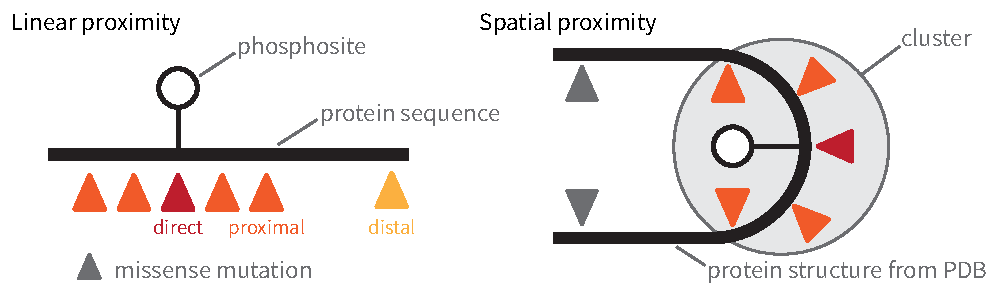
\includegraphics[width=0.9\linewidth]{figures/chap01_intro/ptm_mutational_impact.pdf}
    \caption{Schematic overview of mutational impact on PTM function.}
    \label{fig:intro-ptm-mut-impact}
\end{figure}

% Direct overlap example
Due to the important role of PTMs in cellular signaling, their functions are often perturbed or disrupted in cancer through mutation (\fref{fig:intro-ptm-mut-impact}). The most straightforward effect of a mutation is through its direct overlap with a PTM site on the substrate. The substituted amino acid may not be recognized by the original PTM modifier or might not be modified at all, thus disrupting PTM function. For example, beta-catenin, encoded by \gene{CTNNB1}, is an essential protein in the Wnt signaling pathway regulating cell growth \cite{gaoc_zhangw:ExonMutations2017}. Phosphorylation on its N-terminal domain by GSK3β kinase is required for its degradation via the ubiquitin proteasome pathway \cite{millerjr_moonrt:SignalTransduction1996}. However, hotspot mutations of \gene{CTNNB1} at the N-terminal phosphosites such as S33 and S37 are found in colon, lung, and liver cancers \cite{gaoc_zhangw:ExonMutations2017}. Those mutations potentially disrupt phosphosite-dependent degradation and lead to aberrantly high expression of beta-catenin and uncontrolled cell proliferation.

% Proximal overlap example
A mutation can also substitute the proximal residue of a PTM site, leading to a different PTM abundance level or downstream function change in cancer. For example, aurora kinase B (\gene{AURKB}), a substrate of P-2 arginine \cite{endicottja_johnsonln:StructuralBasis2012}, phosphorylates p53 at the T284 residue and marks p53 for degradation through the ubiquitin proteasome pathway \cite{gullycp_leemh:AuroraKinase2012}. A recurrent mutation in colorectal cancer, \gene{TP53} p.R282W, which changes residue 282 from arginine to tryptophan, has been shown in cell lines to disrupt the T284 phosphorylation by \gene{AURKB} \cite{wagiho_badergd:MIMPPredicting2015}.

To demonstrate the potential impact of mutation and PTM spatial clustering, We developed a tool, HotPho, specifically looking for clusters of mutation and phosphosites on protein structures and identified potentially functional clusters across 5 cancer types \cite{huangk_dingl:SpatiallyInteracting2021}. Taken together, PTM overlapping mutations in cancer have been experimentally shown to disrupt PTM function and abundance. However, PTM abundance was not directly measured in the original cancer samples in the examples above, and the extent of the downstream impact of PTM overlapping mutations is not well understood. By measuring the PTM abundance, gene expression, protein expression, and the mutation profile of the same cancer sample, we will be able to directly observe the PTM overlapping mutations, their impact on a PTM site, and their implication in downstream functions.


\subsection{Large-scale proteomics cancer cohorts by CPTAC}
The Clinical Proteomic Tumor Analysis Consortium (CPTAC) aims to understand the proteogenomic basis of cancer and to accelerate the translation of findings into clinical applications \cite{rodriguezh_lowydr:NextHorizon2021}. CPTAC expands the multi-omics landscape of TCGA to proteins and protein modifications, generating somatic mutation calls, protein expression data, and PTM abundances in paired normal and tumor samples from multiple cancer types. To ensure that the proteomics technology is ready to answer biological questions in a large number of samples, CPTAC has been developed in multiple phases. In the first phase, studies were conducted to evaluate the reproducibility of various mass spectrometry based assays between clinical samples from multiple laboratories \cite{addonata_carrsa:MultisiteAssessment2009,rudnickpa_steinse:PerformanceMetrics2010}. Results showed that mass spectrometry data were reproducible and a strategy was developed to combine the protein and phosphoprotein expressions of multiple experiment runs, allowing the technology to analyze larger sample cohorts. During the second phase of CPTAC, clinical samples of three cancer types were characterized by mass spectrometry assays: colon/rectal cancer (CO) \cite{zhangb_thencicptac:ProteogenomicCharacterization2014}, breast (BRCA) cancer \cite{mertinsp_ncicptac:CPTACBreastCancer2016}, and ovarian cancer (OV) \cite{zhangh_townsendrr:IntegratedProteogenomic2016}. Building upon genomic understanding from previous TCGA studies, CPTAC2 showed the downstream functional impact of the mutations on protein activity in various signaling pathways.

The third and current CPTAC phase, CPTAC3, is exploring the proteogenomic landscape of additional cancer types: clear cell renal carcinoma (ccRCC) \cite{clarkdj_zhangh:IntegratedProteogenomic2019}, uterine corpus endometrial carcinoma (UCEC) \cite{douy_zhaog:CPTACUCEC2020}, lung adenocarcinoma (LUAD) \cite{vasaikars_cptac:ProteogenomicAnalysis2019}, glioblastoma (GBM) \cite{wanglb_cptac:GBM2021}, pancreatic adenocarcinoma (PDAC) \cite{caol_zhaog:ProteogenomicCharacterization2021}, lung squamous cell carcinoma (LSCC) \cite{satpathys_hanhanz:ProteogenomicPortrait2021}, head and neck squamous cell carcinoma (HNSCC) \cite{huangc_zhuj:ProteogenomicInsights2021}, and more. For each cancer type, CPTAC3 will collect around 200 treatment-naive samples and split these samples into discovery and confirmatory cohorts. Besides the phosphoproteome data that previous CPTAC cohorts have generated, studies of many CPTAC cancer types will also provide other PTM enriched MS data, including acetylation, ubiquitination, methylation, and glycosylation.



\section{Glioblastoma}
GBM is the most common primary malignant brain tumor with an incidence of 3.22 per 100,000 persons in the United States, a median survival of less than 2 years from diagnosis18,19 and limited treatment options20,21. TCGA surveyed 206 GBMs with genomic and transcriptomic profiling22, extending the subclassifications developed by Aldape and colleagues23,24. The current view is that IDH-wild type GBMs fall into three distinct subclasses: proneural, classical, and mesenchymal, based on genomic alterations and gene expression signatures22,24–28. The tumor microenvironment may also play an important role in GBM pathogenesis, where tumor-associated macrophages (TAMs) comprise the majority of the immune population29–31. TAMs originate from tissue-resident microglia and bone marrow-derived macrophages (BMDMs), with evidence suggesting that they facilitate tumor proliferation, survival, and migration30. M2-type macrophages, typically thought of as immunosuppressive, dominate and may serve as a microenvironmental advantage to the tumor32.

Despite extensive molecular and immunological characterization of GBM, surgical resection followed by concurrent chemotherapy and radiotherapy remain the standard of care33–35, and targeted therapies have been disappointing so far. Several promising immunotherapies have been proposed, including checkpoint inhibitors, vaccines, Chimeric antigen receptor (CAR) T-cell therapy, and viral therapy, though none have yet demonstrated therapeutic efficacy in phase 3 clinical trials20,21,36. Importantly, the current state of the art method treats all GBM patients uniformly upon diagnosis. No treatment has been found to work in a pre-specified subset of patients based on transcriptomic subtypes. Hence, there is an urgent need for a more nuanced understanding of tumor cells beyond gene expression, and the tumor microenvironment in a manner that is predictive of precision therapy efficacy.

\begin{figure}[tb]
    \centering
    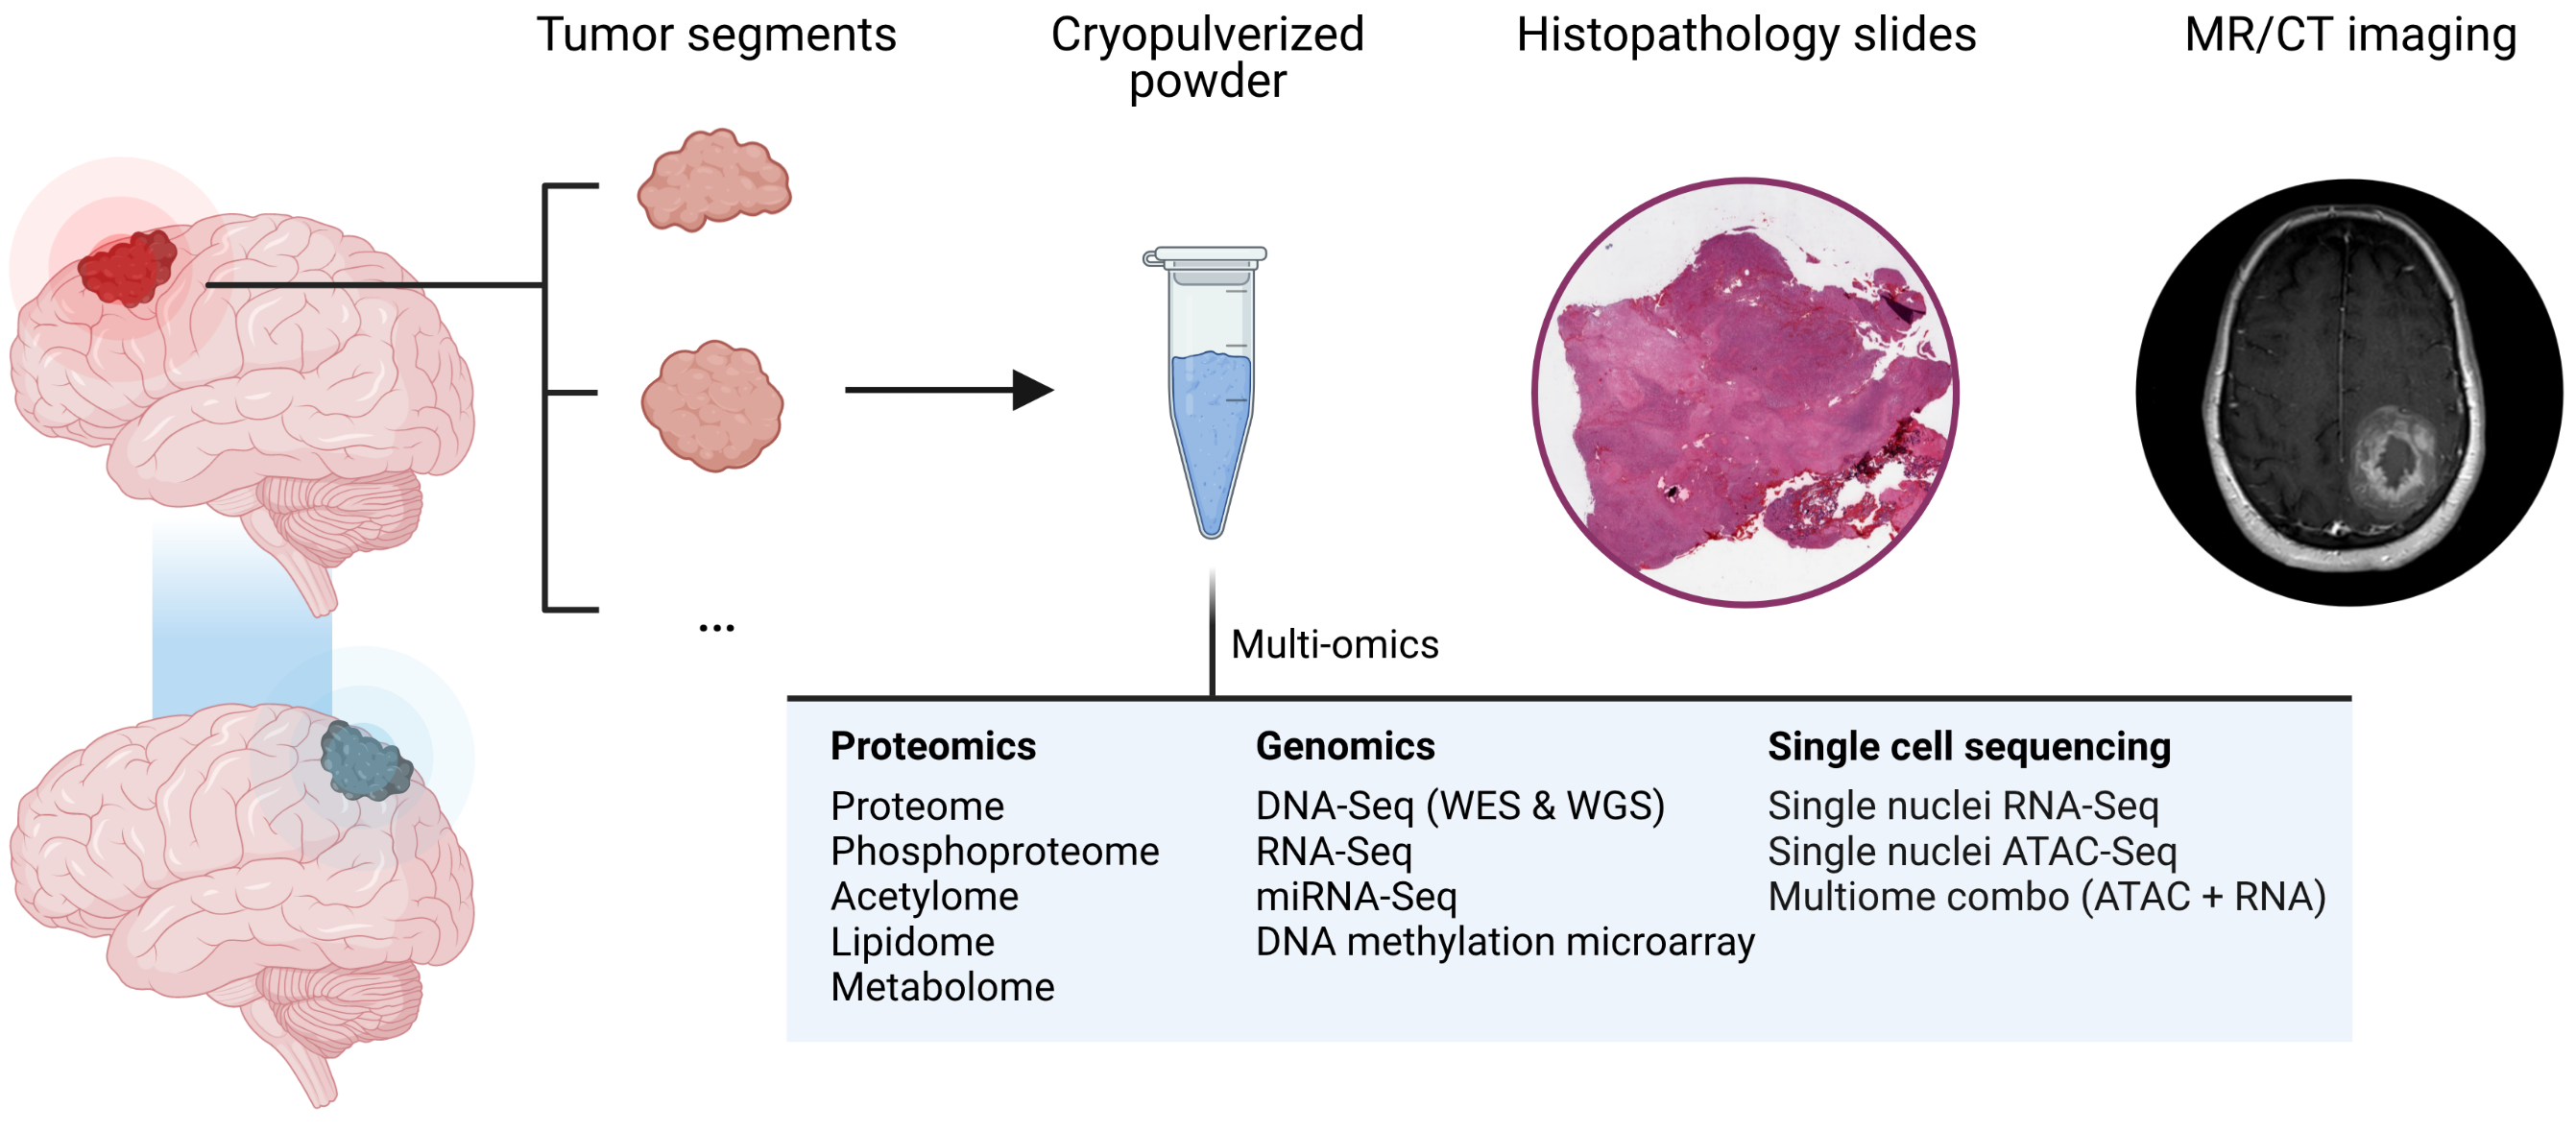
\includegraphics[width=1\linewidth]{figures/chap01_intro/cptac_gbm_multi-omics.png}
    \caption[Overview of the CPTAC GBM data collection and study design.]{%
        Overview of the CPTAC GBM data collection and study design.
        \sourceatright[2em]{\footnotesize Created with BioRender.com}
    }
    \label{fig:intro-cptac-gbm-study-design}
\end{figure}



\defaultlists

\chapter{Mutation Pipeline QC}
\label{chap:mut-pipeline-qc}


\section{Summary}
We present a systematic analysis of the effects of synchronizing a large-scale, deeply characterized, multi-omic dataset to the current human reference genome, using updated software, pipelines, and annotations.
For each of 5 molecular data platforms in The Cancer Genome Atlas (TCGA)---mRNA and miRNA expression, single nucleotide variants, DNA methylation and copy number alterations---comprehensive sample, gene, and probe-level studies were performed, towards quantifying the degree of similarity between the \enquote*{legacy} GRCh37 (hg19) TCGA data and its GRCh38 (hg38) version as \enquote*{harmonized} by the Genomic Data Commons.
We offer gene lists to elucidate differences that remained after controlling for confounders, and strategies to mitigate their impact on biological interpretation.
Our results demonstrate that the hg19 and hg38 TCGA datasets are very highly concordant, promote informed use of either legacy or harmonized omics data, and provide a rubric that encourages similar comparisons as new data emerge and reference data evolve.



\chapter{PTMcosmos}
\label{chap:ptmcosmos}



\section{Summary}
PTMcosmos is a comprehensive database with an interactive web portal designed to catalog and visualize post-translational modifications (PTMs) in humans. It contains 469,183 experimentally-validated PTM sites and their supporting evidence from UniProt Knowledge Base, PhosphoSitePlus, and Clinical Proteomic Tumor Analysis Consortium (CPTAC). PTMcosmos summarizes the entire spectrum of CPTAC proteomics data on human cancer patients, including protein and PTM peptide abundance data from 10 different cancer types. Additionally, PTMcosmos contains cancer somatic mutations from the Cancer Genome Atlas (TCGA), thus allowing for the collective integration and analysis of different data types.  In PTMcosmos, we have built an ensemble of interactive visualization tools that will allow researchers to investigate altered PTM functions due to genetic alterations in close proximity. The database is live at \url{https://ptmcosmos.wustl.edu}. Furthermore, we used PTMcosmos to investigate PTM regulation across cancer types. First, we investigated the differential abundance of the PTM sites of cancer driver genes, focusing primarily on phosphorylation of the tumor suppressor retinoblastoma protein (encoded by \gene{RB1})  and acetylation of the histone acetyltransferase E1A Binding Protein P300 (\gene{EP300}) across cancer types. We analyzed the association between these PTM events and downstream targets, as well as with tumor subtypes, significantly mutated gene (SMG) mutation status  and clinical features. Second, we investigated the association of the protein abundance of cancer driver genes with ubiquitylsites in lung squamous cell carcinoma (LSCC) to nominate potentially novel modes of regulation of these proteins’ activity. We further analyzed the tumor subtype specificity and tumor-normal abundance changes of these ubiquitylsites and their corresponding substrate proteins, identifying several EGFR ubiquitylsites which may regulate EGFR abundance in LSCC. Finally, we identified the linear and spatial clustering of mutations and PTM sites, identifying multiple mutation-PTM clusters in cancer related genes, including TP53, PIK3CA, CTNNB1, EGFR, and IDH1. We envision that PTMcosmos will serve both the CPTAC consortium and the wider research community to better understand the role of PTMs in cancer.


\section{Introduction}
Post-translational modifications (PTMs) act as ``switches'' of protein activity and have been shown to be commonly dysregulated in cancer, controlling the pathway activities and tumor phenotypes \cite{hanahand_weinbergra:HallmarksCancer2011}. Phosphorylation \cite{severr_bruggejs:SignalTransduction2015}, acetylation \cite{dimartilem_trisciuogliod:MultifacetedRole2016,gilj_encarnacion-guevaras:LysineAcetylation2017}, and ubiquitination \cite{dengl_wangp:RoleUbiquitination2020} have all be shown to play distinct roles in tumorigenesis. The known function of the detected PTM sites are curated through a long term effect by databases such as UniProt \cite{theuniprotconsortium_theuniprotconsortium:UniProtWorldwide2019} and PhosphoSitePlus \cite{hornbeckpv_skrzypeke:PhosphoSitePlus2015} by recording the reported publications and validation experiments. PTM dysregulation through mutations in cancer has been actively explored, where linearly and spatially closed mutations could disrupt the PTM site and affect the underlying protein function \cite{reimandj_badergd:MutationalLandscape2013,creixellp_lindingr:KinomewideDecoding2015,wagiho_badergd:MIMPPredicting2015,krassowskim_reimandj:ActiveDriverDBHuman2018,huangk_dingl:SpatiallyInteracting2021}.

Recent advancements in high-throughput multiplexed mass spectrometry have enabled consortia such as Clinical Proteomic Tumor Analysis Consortium (CPTAC) \cite{%
zhangh_townsendrr:IntegratedProteogenomic2016,
rodriguezh_penningtonsr:RevolutionizingPrecision2018,
clarkdj_zhangh:IntegratedProteogenomic2019,
vasaikars_cptac:ProteogenomicAnalysis2019,
douy_zhaog:CPTACUCEC2020,
mcdermottje_rodlandkd:ProteogenomicCharacterization2020,
krugk_zimmermanlj:ProteogenomicLandscape2020,
huy_shiz:IntegratedProteomic2020,
petraliaf_bocikwe:IntegratedProteogenomic2020,
gillettema_shiz:ProteogenomicCharacterization2020,
huangc_zhuj:ProteogenomicInsights2021,
wanglb_cptac:GBM2021,
rodriguezh_lowydr:NextHorizon2021}
and International Cancer Proteogenome Consortium (ICPC) \cite{%
gaoq_fanj:IntegratedProteogenomic2019,
mundg_hwangd:ProteogenomicCharacterization2019,
chenyj_chenyj:ProteogenomicsNonsmoking2020}
to capture tens of thousands of PTM sites across a large number of tumor samples of multiple cancer types. However, several challenges exist to impede a researcher's ability to utilize the large-scale datasets and investigate the PTM sites of interest. It is difficult to integrate the datasets with existing PTM databases due to the annotation differences. The protein sequencing differences used by different projects result in the coordinate change of PTM sites. We previously developed a tool to prioritize the phospho mutation interactions spatially close on 3D protein structures \cite{huangk_dingl:SpatiallyInteracting2021}, however, the interactions of mutation and other PTM types have not been explored. Non-trivial bioinformatic expertise is required to carry out the above analyses.

Here we present PTMcosmos, a comprehensive database for the collection, annotation, and visualization of PTM sites in cancer. This database enables computational and experimental researchers to analyze the abundance, detection rates and supporting evidence of PTM sites, as well as their interplay with mutations in linear and 3D space. Additionally, we demonstrate the utility of PTMcosmos in pan-cancer analyses involving PTM dysregulation through abundance changes and interaction with mutations. We anticipate that PTMcosmos will serve the cancer research community and further our understanding of PTMs in cancer.



\section{Results}

\subsection{Data collection and harmonization}
We developed PTMcosmos, a web portal to provide a comprehensive resource to the proteogenomics community to study cancer \fref{fig:ptmcosmos-workflow}. Total 432,021 PTM sites were collected from two databases, UniProt Knowledge Base and PhosphoSitePlus, and two experimental proteomic consortia across 13 studies and 11 cancer types, CPTAC and ICPC \fref{fig:ptmcosmos-stats-cptac-by-cancer}. To study the mutational impact on PTMs, we also collected the somatic mutations from the matching CPTAC tumor samples and a pan-cancer collection from TCGA MC3 project \cite{ellrottk_tcga:MC3MutationCalling2018}. Additional protein annotations were loaded to bridge the proteins with their known biological functions, including the non redundant protein sequence archive from UniPar \cite{leinonenr_apweilerr:UniProtArchive2004}, standardized gene symbol, aliases and identifiers from HUGO Gene Nomenclature Committee (HGNC) \cite{brufordea_tweedies:GuidelinesHuman2020}, protein structures from Protein Data Bank (PDB) \cite{bermanhm_bournepe:ProteinData2000}, protein domains from InterPro \cite{blumm_finnrd:InterProProtein2021} and Pfam \cite{mistryj_batemana:PfamProtein2021}, and protein pathways and complexes from OmniPath \cite{tureid_saez-rodriguezj:OmniPathGuidelines2016}.

\begin{figure}[tb]
    \centering
    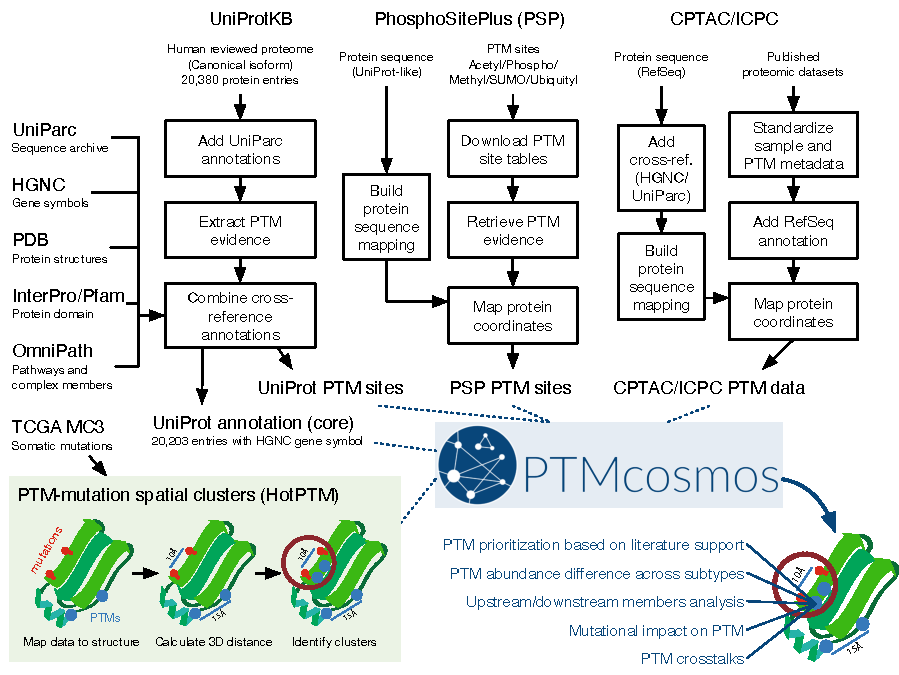
\includegraphics[width=0.9\linewidth]{figures/chap03_ptmcosmos/figure1_ptmcosmos_workflow.pdf}
    \caption[PTMcosmos overview.]{PTMcosmos overview.}
    \label{fig:ptmcosmos-workflow}
\end{figure}

To avoid ambiguous PTM location due to multiple protein sequence versions, we keep track of the underlying peptide sequences of the PTM sites and harmonized. We used UniProt Archive (UniParc) \cite{leinonenr_apweilerr:UniProtArchive2004} to check for sequence identity and performed global protein sequence alignment to mapped all the reported PTM sites to UniProt canonical protein isoforms (release 2021.02) (\fref{fig:ptmcosmos-map-stats-schematic}; Methods). For PhosphoSitePlus whose sequences are mostly based on UniProt, over 99.9\% of the PTM sites were reported on the proteins identical to UniProt. Only 0.3\% of them (n = 1,060) changed their coordinates after the mapping and only 0.01\% of them (n = 33) failed to be mapped to UniProt. Across the experiment cohorts where RefSeq protein sequences were used in the data generation (\tref{tab:ptmcosmos-peptide-db}), about 60--75\% of the PTM sites are reported on the identical protein sequences to UniProt, while 10--20\% of them changed their coordinates after the mapping and 1--3\% of them are not mappable (\fref{fig:ptmcosmos-map-stats-acetyl}--\subcaptionref{fig:ptmcosmos-map-stats-phospho}).

\begin{figure}[tbp]
    \centering
    \phantomlabel{fig:ptmcosmos-map-stats-schematic}
    \phantomlabel{fig:ptmcosmos-map-stats-acetyl}
    \phantomlabel{fig:ptmcosmos-map-stats-ubiquityl}
    \phantomlabel{fig:ptmcosmos-map-stats-phospho}
    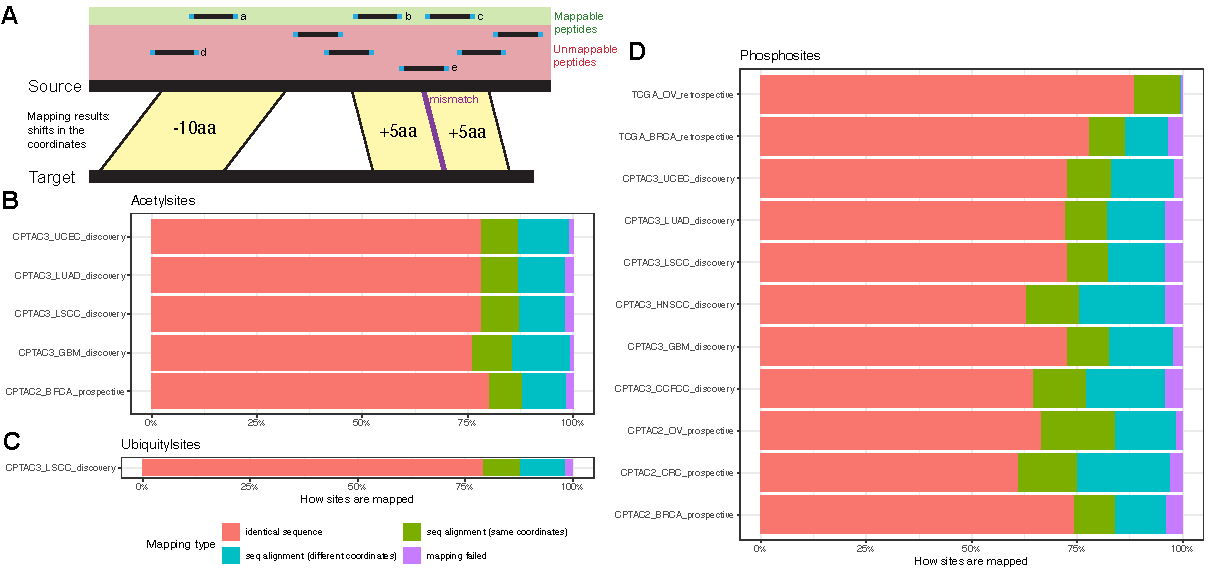
\includegraphics[width=\linewidth]{figures/chap03_ptmcosmos/figures1_mapping_stats.pdf}
    \caption[Supporting details of the peptide re-annotation and coordinate mapping.]{%
        Supporting details of the peptide re-annotation and coordinate mapping.
        \subref{fig:ptmcosmos-map-stats-schematic}
        A schematic representation of the peptide coordinate mapping using global protein sequence alignment. Peptides (a--e) including the flanking sequence are the PTM sites to be mapped. Only peptides (a--c) in the yellow regions produced by the sequence alignment are mappable. Peptide d is not mappable since only a parital of its sequence can be aligned. Peptide e is also not mappable due to a mismatch between the source and target protein sequences. PTM peptides mapability of \subref{fig:ptmcosmos-map-stats-acetyl} acetylation,
        \subref{fig:ptmcosmos-map-stats-ubiquityl} ubiquitination,
        \subref{fig:ptmcosmos-map-stats-phospho} phosphorylation CPTAC proteome datasets.
    }
    \label{fig:ptmcosmos-map-stats}
\end{figure}

By combining all the data sources and annotations. a total of 3.1 millions exhibits of PTM supporting evidences are collected from over 75 thousands of publications and other kinds of experimental validations in the database (\fref{fig:ptmcosmos-stats-publications-per-ptm}, \ref{fig:ptmcosmos-stats-publications-per-year}). The majority of PTM sites received 1--5 supporting publications, where the phosphosites are much more investigated and reported than other PTM types. Surprisingly, still a large number (> 20\%) of PTM sites have low to no literature support. Thanks to the massive effort of literature curation by UniProt and PhosphoSitePlus, the collected literature can be dated back to 1980s. Research of earlier days focused on the characterization of small number of PTM sites, whereas many new PTM sites were discovered using the high throughput methods.

\begin{figure}[tbp]
    \centering
    \phantomlabel{fig:ptmcosmos-stats-cptac-by-cancer}
    \phantomlabel{fig:ptmcosmos-stats-publications-per-ptm}
    \phantomlabel{fig:ptmcosmos-stats-publications-per-year}
    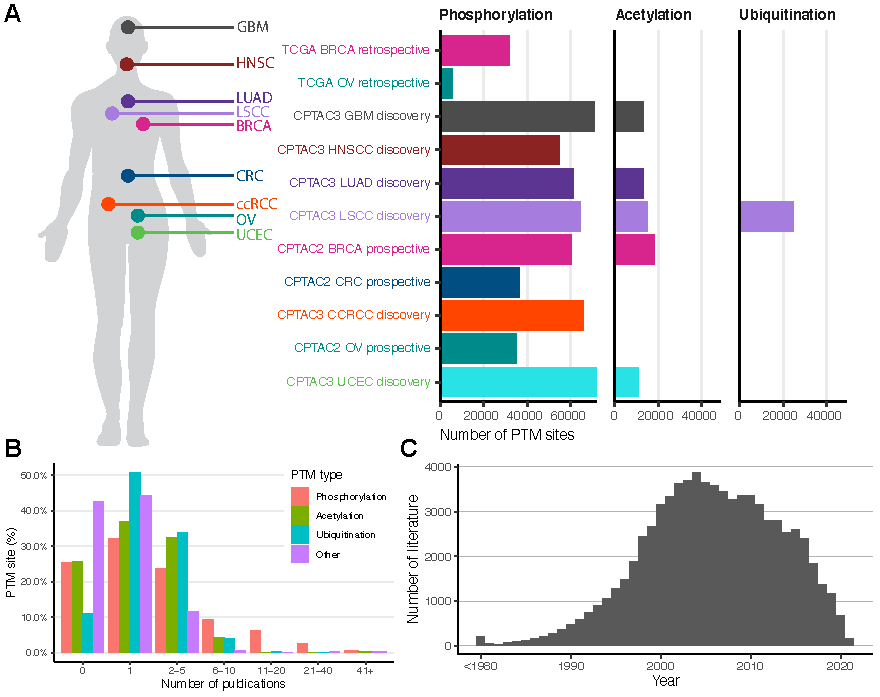
\includegraphics[width=\linewidth]{figures/chap03_ptmcosmos/figure1_ptmcosmos_stats.pdf}
    \caption[Overview of experiment proteome datasets and distribution of PTM supporting evidence collected in PTMcosmos.]{%
        Overview of experiment proteome datasets \subref{fig:ptmcosmos-stats-cptac-by-cancer} and distribution of PTM supporting evidence collected in PTMcosmos.
        \subref{fig:ptmcosmos-stats-publications-per-ptm}
        Distribution of supporting publications per PTM type.
        \subref{fig:ptmcosmos-stats-publications-per-year}
        Distribution of supporting publications along its publication time.
    }
    \label{fig:ptmcosmos-stats}
\end{figure}


\subsection{Descriptive analysis of PTM sites in PTMcosmos}
We analyzed the PTM sites in PTMcosmos to understand the pathways and domains present in the database. All 50 cancer hallmark pathways were represented in PTMcosmos, with phosphorylation being the dominant PTM for each pathway (\fref{fig:ptmcosmos-site-detail-pathway-domain}). The mitotic spindle, G2/M checkpoint and E2F pathways displayed the largest number of PTM sites, while pancreas beta cells, Notch signaling and angiogenesis showed the lowest number of PTM sites. To understand these results in greater detail, we investigated the genes and domains represented among PTM sites in the top three pathways. Consistent with their presence in cytoskeletal proteins, spectrin and filamin repeats had the highest number of PTMs (n = 655; 639) in the mitotic spindle pathway, with phosphorylation being the dominant PTM among these domains (n = 283; 390). The RecF/RecN/SMC N terminal domain, found in structural maintenance of chromosomes (SMC) proteins, was highly abundant in both the G2/M checkpoint (n = 342) and E2F target pathways (n =4 68), with ubiquitination being the dominant modification in this domain (n = 165; 194). The protein kinase domain, modified predominantly by ubiquitination and phosphorylation, was the most represented domain among G2/M checkpoint pathway members (151 phospho- and 141 ubiquitylsites out of 343 PTM sites).

\begin{figure}[tbp]
    \centering
    \phantomlabel{fig:ptmcosmos-site-detail-venn}
    \phantomlabel{fig:ptmcosmos-site-detail-pathway-domain}
    \phantomlabel{fig:ptmcosmos-site-detail-phspho-tyr}
    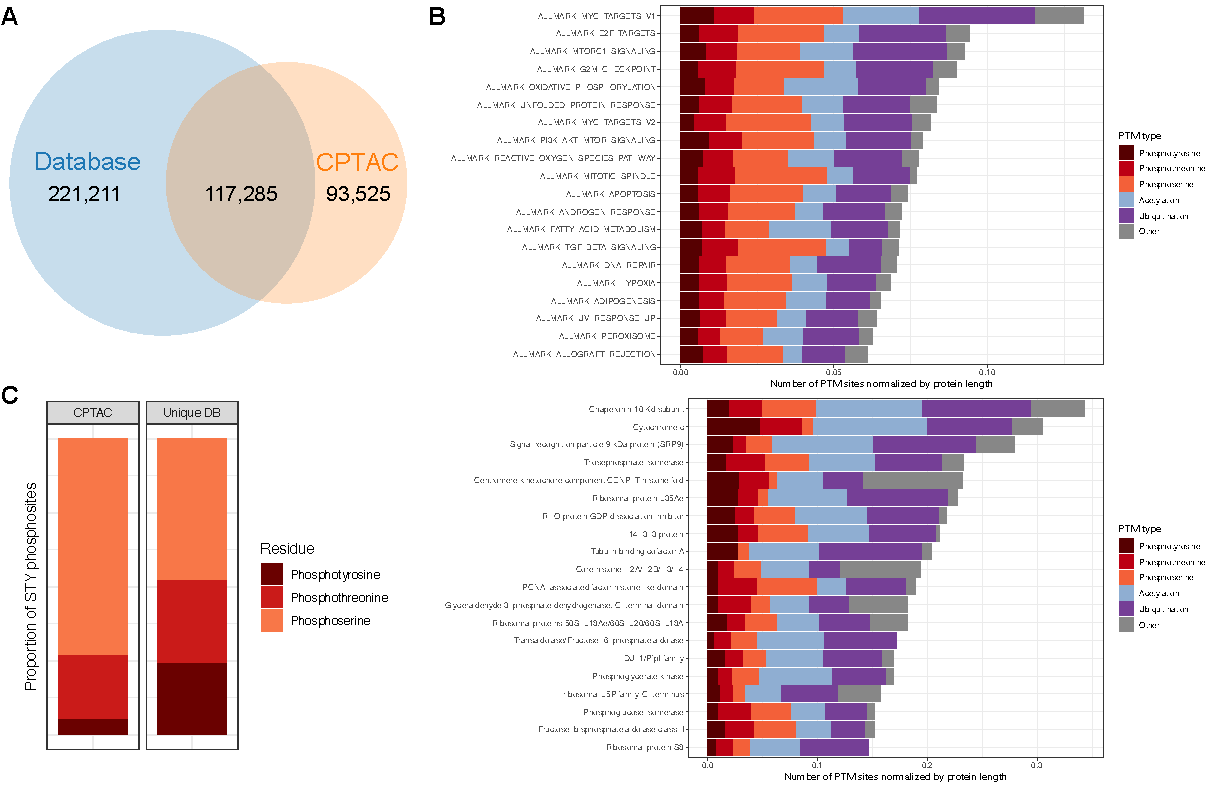
\includegraphics[width=\linewidth]{figures/chap03_ptmcosmos/figure2_ptmcosmos_site_detail.pdf}
    \caption[Descriptive analysis of the PTM sites in PTMcosmos.]{%
        Descriptive analysis of the PTM sites in PTMcosmos.
        \subref{fig:ptmcosmos-site-detail-venn}
        Venn diagram showing unique CPTAC and database sites. Database sites are only found in alternative evidence sources (PhosphoSitePlus and UniProtKB).
        \subref{fig:ptmcosmos-site-detail-pathway-domain}
        The top Hallmark pathways and PFAM domains (Y axis) represented among all PTM sites in PTMcosmos. For each pathway or domain, the number of PTM sites (X axis) is normalized by the total protein sequence length of entries in the given pathway or domain.
        \subref{fig:ptmcosmos-site-detail-phspho-tyr}
        The proportion of tyrosine phosphosites present among all CPTAC sites compared to sites uniquely present in PhosphositePlus or UniProtKB (referred to as ``unique DB'' sites).
    }
    \label{fig:ptmcosmos-site-detail}
\end{figure}

Next, we investigated the PTM sites detected only in CPTAC and those found only in alternative evidence sources (PhosphoSitePlus and UniProtKB). In total, 93,319 PTM sites were unique to CPTAC experiments (hereafter called unique CPTAC sites), while 258,935 sites were detected in PhosphoSitePlus or UniProtKB, but not CPTAC (hereafter called unique database sites) (\fref{fig:ptmcosmos-site-detail-venn}).
Among all the Pfam protein domains tested (n=2,501),  248 domains were significantly enriched among the unique database sites, including ``zinc finger, C2H2 type'' (FDR = 3.84e-147), ``cadherin domain'' (FDR = 3.08e-127), ``core histone H2A/H2B/H3/H4'' (FDR = 7.13e-90), ``immunoglobulin V-set domain'' (FDR = 2.53e-56) and “protein kinase domain” (FDR = 2.33e-53).
Four hallmark pathways were significantly enriched among the unique database sites: ``HALLMARK\_INFLAMMATORY\_RESPONSE'' (FDR = 3.10e-32), ``HALLMARK\_SPERMATOGENESIS'' (FDR = 3.94e-31), ``HALLMARK\_IL6\_JAK\_STAT3\_SIGNALING'' (FDR = 3.01e-10) and ``HALLMARK\_NOTCH\_SIGNALING'' (FDR = 9.83e-05).
Similarly, 75 protein domains were significantly enriched among unique CPTAC sites, with the five most significantly enriched domains being ``spectrin repeat'' (FDR = 1.15e-73), ``lipocalin/cytosolic fatty-acid binding protein family'' (FDR = 7.33e-35), ``serpin (serine protease inhibitor)'' (FDR = 3.04e-23), ``apolipoprotein A1/A4/E domain'' (FDR = 3.31e-20) and ``transferrin'' (FDR = 1.72e-18).
Seven hallmark pathways were significantly enriched among unique CPTAC sites, with the top five pathways being ``HALLMARK\_COAGULATION'' (FDR = 1.05e-83), ``HALLMARK\_EPITHELIAL\_MESENCHYMAL\_TRANSITION'' (FDR = 1.75e-62), ``HALLMARK\_KRAS\_SIGNALING\_DN'' (FDR = 8.38e-29), ``HALLMARK\_COMPLEMENT'' (FDR = 4.55e-19) and ``HALLMARK\_ANGIOGENESIS'' (FDR = 3.28e-13).
Interestingly, among serine, threonine and tyrosine phosphosites, unique database phosphosites were enriched for phosphotyrosine compared to all CPTAC sites (OR = 0.17, p < 2.2e-16) (\fref{fig:ptmcosmos-site-detail-phspho-tyr}), suggesting a potential limitation of mass spectrometry technology in detecting phosphotyrosine.


\subsection{PTMcosmos user interface}
To facilitate a friendly user interface, we made all the information searchable on PTMcosmos in a similar design as UniProt (\fref{fig:ptmcosmos-usage-demo}). Users are able to query the gene and protein name of interest and the PTM information is organized on a protein basis. The page contains a protein feature viewer to show the location of PTM sites and protein domain along its sequence. For each PTM site, its supporting evidence is grouped into dropdown menus based on the evidence source and type. Details of each evidence exhibit is available in the dropdown menu, including the publication information, sequence similarity source, and the experiment cohorts detecting the site. For PTM sites with experiment datasets loaded in PTMcosmos, an additional interactive page is available for users to explore the PTM abundance in the dataset. For proteins with mutation and PTM spatial clusters reported by HotPTM, an interactive viewer is available for users to explore the protein structure annotated with the PTM-mutation clusters.

\begin{figure}[tb]
    \centering
    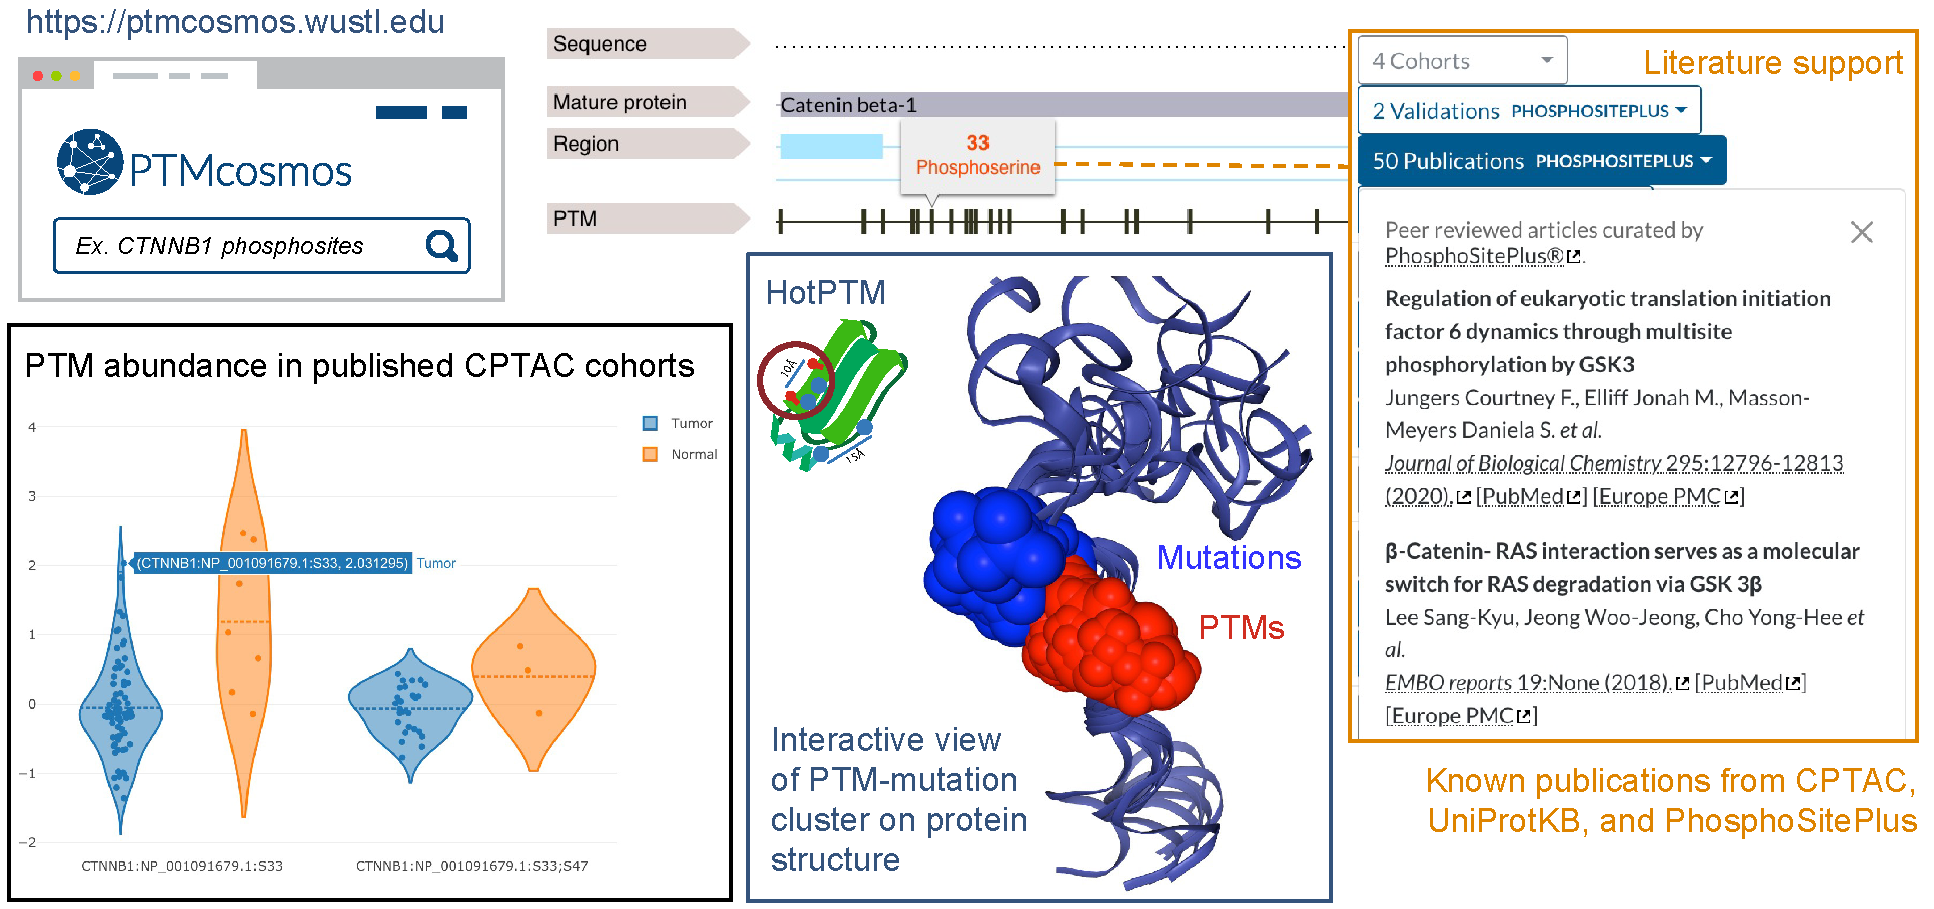
\includegraphics[width=\linewidth]{figures/chap03_ptmcosmos/figure3_ptmcosmos_usage.pdf}
    \caption[PTMcosmos usage demonstration.]{%
        PTMcosmos usage demonstration using β catenin phosphosites as an example. From right to left, the phosphosite S33, from the literature, is known to regulate the degradation of itself. The mutational impact analysis by HotPTM shows that endometrial cancer samples frequently harbor nearby mutations that disrupt this phosphosite. Finally, users can quickly check the relative abundance change at peptide level in every published CPTAC cohort.
    }
    \label{fig:ptmcosmos-usage-demo}
\end{figure}


\subsection{Differential expressed PTM sites between tumor and normal samples across cancer types}
To showcase how PTMcosmos can help research investigate PTM's function in cancer,  we examined PTM sites differentially expressed between tumor and normal adjacent tissue samples. To uncover functionally relevant PTM sites, we restricted our analysis to PTMs of 188 known cancer driver genes, 180 of which had PTM sites detected in the CPTAC cohorts \cite{baileymh_dingl:ComprehensiveCharacterization2018}. We found a total of 2,055 differentially expressed PTM sites across 146 driver genes, consisting of 1,405 phosphosites and 522 acetylsites (\fref{fig:ptmcosmos-de-overview}). To further prioritize functional PTM sites, we used PTMcosmos to select for sites detected in previous studies. Several driver genes showed differential acetylation and phosphorylation across cancer types. CDK12 and EZH2 phosphorylation were upregulated across the same six cancer types (UCEC, OV, LUAD, LSCC, GBM, and CRC). Acetylation and phosphorylation of the cell cycle protein nucleophosmin (NPM1) was consistently upregulated in LUAD and LSCC, with the NPM1-T199 phosphosite, known to play a role in the DNA damage response, also had enriched detection in LSCC tumors compared to normal adjacent tissue. The chromatin remodelling protein BRG1 (SMARCA4) also showed increased phosphorylation across multiple cancer types, including LSCC and LUAD. Notably, four cancer types showed upregulated acetylation of the histone acetyltransferase p300, and eight cancer types displayed increased phosphorylation of the canonical tumor suppressor Rb.

\begin{figure}[p]
    \centering
    \phantomlabel{fig:ptmcosmos-de-overview}
    \phantomlabel{fig:ptmcosmos-ep300-prot-paint}
    \phantomlabel{fig:ptmcosmos-ep300-hist-acetyl}
    \phantomlabel{fig:ptmcosmos-ep300-assoc}
    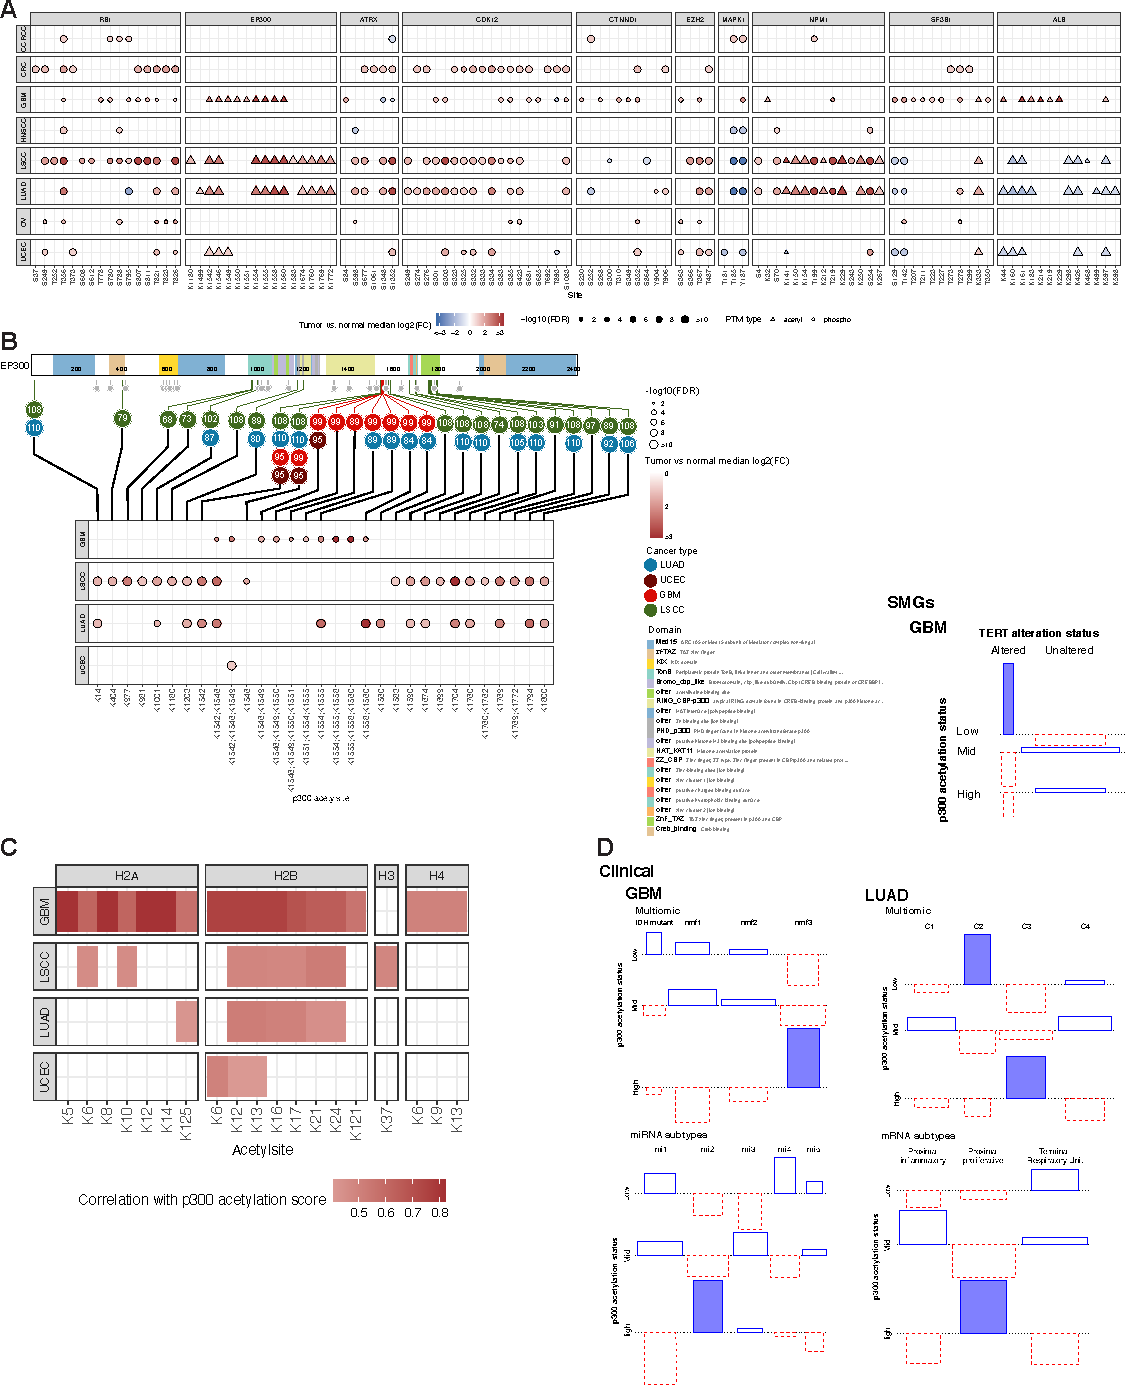
\includegraphics[width=\linewidth]{figures/chap03_ptmcosmos/figure4_ptmcosmos_ep300.pdf}
    \caption[Differential expression analysis of sites in PTMcosmos.]{%
        Differential expression analysis of sites in PTMcosmos.
        \subref{fig:ptmcosmos-de-overview}
        Overview of differentially expressed driver gene acetyl- and phosphosites across 8 cancer types.
        \legendcontdnote
    }
    \label{fig:ptmcosmos-ep300}
\end{figure}
\begin{figure}[t]
    \centering
    \legend{%
        \legendcontdref{fig:ptmcosmos-ep300}
        \subref{fig:ptmcosmos-ep300-prot-paint}
        Differentially expressed acetylsites of the acetyltransferase p300 mapped onto the protein's domain structure. The numbers shown in the circles represent the number of samples in a cohort detecting the given acetylsite.
        \subref{fig:ptmcosmos-ep300-hist-acetyl}
        Heatmap showing the significant Pearson correlations between the aggregate p300 acetylation score and histone acetylsites.
        \subref{fig:ptmcosmos-ep300-assoc}
        Mosaic plot showing the associations between p300 acetylation status and categorical variables such as tumor subtypes and the alteration status of significantly mutated genes.
    }
\end{figure}


\subsection{Tumor-normal comparison of p300 phosphosites}
We observed increased acetylation of the histone acetyltransferase (HAT) p300 across cancer types (\fref{fig:ptmcosmos-ep300-prot-paint}). Autoacetylation of p300 at distinct lysine residues in the HAT domain is known to increase its catalytic activity, with multiple cancer types displaying upregulation of these acetylsites \cite{thompsonpr_colepa:RegulationP3002004}. UCEC tumors showed increased acetylation at the HAT domain residues K1542, K1546 and K1549, while GBM tumors showed upregulated acetylation at multiple additional HAT domain acetylsites spanning residues K1542 to K1560. LSCC and LUAD tumors shared several differentially upregulated p300 acetylsites characterized in previous studies, including the HAT domain sites K1542 and K1546, the E1A adenovirus binding region sites K1674 and K1794, and the K1760 acetylsite, which may function in cytoplasmic signaling \cite{thompsonpr_colepa:RegulationP3002004,zhangt_zhangf:ING5Differentially2018,grimesm_combm:IntegrationProtein2018}. LUAD tumors showed increased acetylation at additional HAT domain sites known to increase enzymatic activity of p300 \cite{thompsonpr_colepa:RegulationP3002004}. These results indicate both cancer type-specific and shared profiles of p300 acetylation.

Because of the role of p300 acetylation in promoting its HAT activity, we hypothesized that p300 acetylation in the HAT domain would correlate with histone acetylation. To investigate this, we computed an aggregate p300 acetylation score through averaging the abundances of known HAT domain acetylsites \cite{thompsonpr_colepa:RegulationP3002004}. As expected, for each cohort of interest the p300 acetylation score was significantly higher in tumor samples compared to NAT. UCEC tumors showed significant correlations between p300 acetylation and H2B acetylation at the N-terminal sites K6, K12 and K13, consistent with N-terminal H2B acetylation being a strong marker for p300 catalytic activity \cite{weinertbt_chunaramchoudhary:TimeResolvedAnalysis2018}. Similarly, in both LSCC and LUAD tumors p300 acetylation was significantly associated with H2B acetylation at residues spanning K12 to K24. LSCC tumors also showed significant correlations between p300 acetylation and N-terminal H2A.X and H2A acetylation. Interestingly, in LSCC tumors, p300 acetylation was also correlated with H3.1 acetylation at K37, although this site has not been found to be acetylated by p300. Similar to other cancer types, GBM tumors showed significant associations between p300 acetylation and N-terminal H2B acetylation at residues spanning K6 to K24. Acetylation at N-terminal sites of H2A.V (K5 to K14) and H2A.X (K6 and K10) was also correlated with p300 acetylation in GBM tumors. Interestingly, GBM tumors displayed strong correlations between N-terminal H4 acetylation (at K6, K9 and K13) and p300 acetylation, consistent with p300 regulating H4 acetylation, although to a lesser degree than H2B acetylation \cite{weinertbt_chunaramchoudhary:TimeResolvedAnalysis2018}. As expected, across cancer types p300 acetylation was significantly correlated with acetylation of its homologue CBP along the activation loop in its HAT domain, which similarly undergoes autoacetylation to promote HAT activity \cite{parks_wrightpe:RoleCBP2017}.

We investigated the effect of p300 acetylation on gene expression programs across cancer types due to its known ability to alter chromatin structure and transcriptional regulation. For each cancer type, we divided samples into p300 acetylation high (>75\% percentile of p300 acetylation score) and low groups (<25\% percentile of p300 acetylation), and explored the differentially expressed genes (DEGs) upregulated in p300 acetylation-high samples. Interestingly, these DEGs were significantly enriched for E2F target genes in LUAD, LSCC and GBM tumors, consistent with previous studies showing that p300/CBP HAT activity is crucial for activating E2F transcriptional programs \cite{ait-si-alis_harel-bellana:CBPP3002000}. These results suggest that in these cancer types, p300 autoacetylation may increase its HAT activity, thus promoting E2F activity. Intriguingly, p300 acetylation was significantly correlated with Rb phosphorylation across GBM tumors. Previous studies have shown that silencing p300 results in decreased phospho-Rb and E2F target gene expression, suggesting that in GBM tumors p300 acetylation and Rb phosphorylation may together regulate E2F transcriptional programs \cite{fauquierl_vandell:CBPP3002018}. Thus, our analysis suggests that p300 autoacetylation may promote E2F activity across cancer types.

Next, we investigated the possible mechanisms regulating p300 acetylation across cancer types. Interestingly, in LUAD tumors p300 protein abundance was strikingly upregulated in tumor samples compared to NAT. Similarly, GBM tumors showed upregulated p300 protein abundance, but no significant difference in p300 protein abundance was observed between UCEC tumors and NAT. Across cancer types, p300 acetylation was significantly correlated with p300 protein abundance, consistent with autoacetylation of p300.

Finally, we explored the association of subtype and clinical data with p300 acetylation. Consistent with the observation of E2F enrichment in p300 acetylation-high tumors, p300 acetylation was significantly associated with the proximal-proliferative subtype and C3 NMF consensus cluster in LUAD, with both groups enriched for cell cycle pathways \cite{gillettema_shiz:ProteogenomicCharacterization2020}. Consistently, previous studies have found that p300 promotes cell proliferation in non-small cell lung cancer cell lines, suggesting that p300, and p300 acetylation, may play a similar role in this cohort \cite{reng_zhaok:CTCFMediatedEnhancerPromoter2017}. Interestingly, across LSCC tumors p300 acetylation was negatively associated with the immune hot subtype and the secretory subtype, and positively associated with the wound healing immune subtype, although the specific biological role of p300 in the immune response in LSCC is unclear. GBM tumors showed positive associations between p300 acetylation and the classical-like nmf3 subtype, consistent with recent proteogenomic studies showing that H2B acetylation is driven in part by p300 in classical-like GBM tumors \cite{wanglb_cptac:GBM2021} (\fref{fig:gbm-histone-acetyl}). High p300 acetylation was also positively associated with the mi2 microRNA cluster in GBM, consistent with this cluster being significantly associated with the classical-like nmf3 cluster \cite{wanglb_cptac:GBM2021} (\fref{fig:gbm-overview-multi-omics}). We also investigated the associations between significantly mutated genes and p300 acetylation across cancer types. In UCEC tumors, CTCF mutations were significantly associated with high p300 acetylation, consistent with previous studies finding that chromatin binding sites for p300 and CTCF interact \cite{houx_zhangl:P300Promotes2018}.


\subsection{Tumor-normal comparison of Rb1 phosphosites}
We observed the upregulation of multiple Rb phosphosites across 8 cancer types (OV, CRC, LSCC, LUAD, GBM, UCEC, HNSCC, CCRCC) known to disrupt the Rb-E2F interaction, thus promoting E2F transcriptional activity and cell cycle progression \cite{rubinsm_rubinsm:DecipheringRetinoblastoma2013} (\fref{fig:ptmcosmos-rb1-prot-paint}).  Interestingly, phosphorylation of Rb at T356, known to promote an order-to-disorder transition in the RbN domain, was significantly upregulated across six cancer types \cite{rubinsm_rubinsm:DecipheringRetinoblastoma2013}. We found that in CPTAC tumors, OV and HNSCC tumors showed increased Rb phosphorylation at S788, while LSCC and GBM tumors exhibited upregulated phosphorylation at S795, with both sites known to in part disrupt binding between E2F and the C-terminal domain of Rb (RbC) \cite{rubinsm_pavletichnp:StructureRb2005}. Dual phosphorylation of Rb at T821 and T826 was increased in LUAD, LSCC and CRC tumors. Phosphorylation of Rb at T373, known to completely inactivate Rb, was upregulated in CRC and UCEC tumors. These results indicate both unique and shared Rb phosphosites across cancer types with functional significance.

\begin{figure}[p]
    \centering
    \phantomlabel{fig:ptmcosmos-rb1-prot-paint}
    \phantomlabel{fig:ptmcosmos-rb1-e2f}
    \phantomlabel{fig:ptmcosmos-lscc-ubiquityl}
    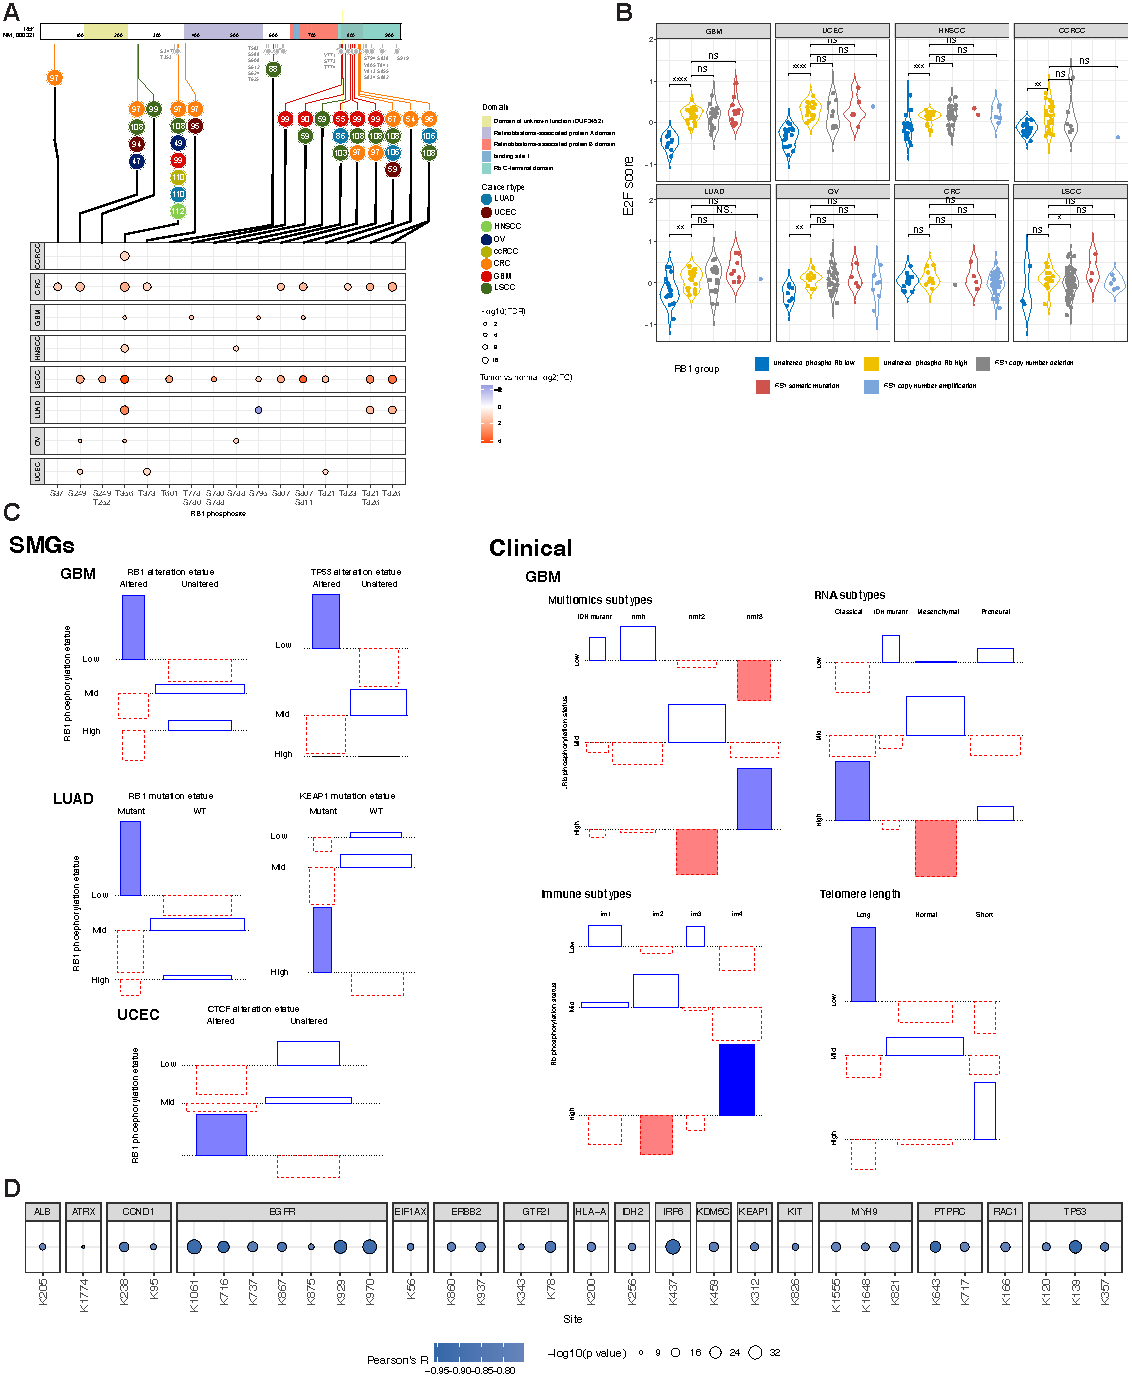
\includegraphics[width=\linewidth]{figures/chap03_ptmcosmos/figure5_ptmcosmos_rb1.pdf}
    \caption[Pan-cancer Rb phosphorylation analysis and LSCC ubiquitination analysis.]{%
        Pan-cancer Rb phosphorylation analysis and LSCC ubiquitination analysis.
        \legendcontdnote
    }
    \label{fig:ptmcosmos-rb1}
\end{figure}
\begin{figure}[t]
    \centering
    \legend{%
        \legendcontdref{fig:ptmcosmos-rb1}
        \subref{fig:ptmcosmos-rb1-prot-paint}
        Overview of differentially expressed Rb phosphosites across 8 cancer types and the mapping of these phosphosites onto the domain structure of Rb. The numbers shown in circles represent the number of samples in the given cohort detecting a phosphosite.
        \subref{fig:ptmcosmos-rb1-e2f}
        Averaged expression of E2F target genes (``E2F score'') stratified by \gene{RB1} alteration status or Rb phosphorylation status.
        \subref{fig:ptmcosmos-lscc-ubiquityl}
        Correlation in lung squamous cell carcinoma between normalized ubiquitylsite abundance and cognate protein abundance for cancer driver genes.
    }
\end{figure}

Due to the importance of Rb phosphorylation in regulating the Rb-E2F interaction, we calculated the E2F transcriptional activity score across cancer types based on gene expression and found it was highly correlated with Rb phosphorylation. Rb-T356 phosphorylation was strongly correlated with E2F activity in ccRCC, GBM and LUAD tumors, suggesting a possible role for this site in the Rb-E2F interaction. We also observed site- and cancer type-specific associations between Rb phosphorylation and E2F activity. Phosphorylation of Rb at T373 was significantly correlated with E2F activity in UCEC tumors. Dual phosphorylation at S807/S811 and T823/T826 were also significantly associated with E2F activity in UCEC and GBM tumors. ccRCC tumors showed strong correlations between Rb-T252 phosphorylation and E2F activity.

Next, we investigated the effect of Rb genetic alterations on the relationship between Rb phosphorylation and E2F activity. We divided tumor samples into an Rb altered group, consisting of samples with either \gene{RB1} somatic mutations or copy number loss, and an Rb unaltered group lacking such alterations. Interestingly, unaltered samples showed stronger associations between Rb phosphorylation and E2F activity, including associations not observed when computing correlations across all tumor samples. GBM unaltered tumors showed significant correlations between E2F activity and Rb-S612 phosphorylation, known to disrupt the E2F binding cleft in the Rb pocket domain \cite{macdonaldji_dickfa:PosttranslationalModifications2012}. Significant correlations for Rb-S788 were also observed in GBM unaltered tumors. LUAD unaltered tumors exhibited a significant correlation between E2F activity and Rb-T821/T826 phosphorylation, known to disrupt the RbC-E2F interaction through promoting binding of RbC to the pocket domain of Rb \cite{rubinsm_pavletichnp:StructureRb2005}. Additionally, LUAD unaltered tumors showed a strong association between Rb-T356 phosphorylation and E2F activity, consistent with our observations in ccRCC, GBM and UCEC. These results suggest that 1) cancer types may utilize distinct Rb phosphosites across domains to promote E2F activity and 2) tumors lacking classical \gene{RB1} genetic alterations may utilize Rb phosphorylation to drive E2F activity. We further investigated the interplay of \gene{RB1} genetic alterations and Rb phosphorylation by comparing E2F activity between unaltered and altered samples. As expected, unaltered phospho-high tumors and altered tumors both showed significantly increased E2F activity when compared to unaltered phospho-low tumors across cancer types. Strikingly, no significant difference in E2F activity was observed when comparing unaltered phospho-high tumors and altered tumors, suggesting that tumors without genetic alterations in \gene{RB1} may utilize Rb phosphorylation to achieve similar levels of E2F activity to \gene{RB1} altered tumors.

Additionally, we investigated the possible mechanisms underlying increased Rb phosphorylation across cancer types. First, we used multi-omics data to investigate the correspondence between \gene{RB1} RNA expression, Rb protein abundance, and Rb phosphorylation. As expected, LUAD tumors showed significantly decreased \gene{RB1} RNA expression compared to normal adjacent tissue (NAT). Interestingly, LUAD tumors showed no significant difference in total protein abundance compared to NAT, but significant upregulation of Rb phosphorylation, suggesting that Rb phosphorylation is regulated independently of \gene{RB1} expression and total Rb protein abundance in LUAD. Intriguingly, UCEC and ccRCC tumors showed global upregulation of \gene{RB1} RNA, Rb protein and phosphorylation abundance. Unlike previous studies implicating \gene{RB1} copy number amplification in contributing to increased Rb phosphorylation in tumors, upregulated \gene{RB1} expression did not appear to be due to copy number amplification in these cohorts \cite{vasaikars_cptac:ProteogenomicAnalysis2019}. These results suggest that LUAD tumors may utilize a distinct mechanism from UCEC and ccRCC tumors in regulating Rb phosphorylation.

To further characterize the regulation of Rb phosphorylation, we investigated the relationship between Rb phosphorylation and cyclin-dependent kinases (Cdk) across cancer types. LUAD tumors showed significant correlations between CDK1 protein abundance and phosphorylation of Rb at S249, T356 and the dual phosphorylation sites T821 and T826, with CDK1 being a putative in vivo kinase of S249 phosphorylation \cite{hasslerm_mittnachts:CrystalStructure2007}. Similarly, in ccRCC tumors, CDK1 protein abundance was strongly correlated with phosphorylation at S249 and T373, both of which are putative CDK1 sites (PSP). ccRCC tumors also showed a strong and significant correlation between Rb-T356 phosphorylation and CDK1 protein abundance, although this phosphosite is not known to be phosphorylated by CDK1. In UCEC tumors, Rb phosphorylation at the putative CDK1/CDK2 sites of S807/S811 and T373 were significantly correlated with both CDK1 and CDK2 protein abundance (PSP). Additionally, phosphorylation at the putative CDK2 phosphosite T356 was strongly associated with CDK2 protein abundance across UCEC tumors. GBM tumors exhibited strong correlations between the protein abundance of the canonical Rb kinase CDK6 and multiple Rb sites, including the known CDK6 site S780 (dually phosphorylated with T778) and the putative CDK6 sites S612, S788, S795, S807, S811 and T826 (dually phosphorylated with T823).  Similar to other cancer types, GBM tumors also showed significant correlations between CDK1 protein abundance and multiple Rb phosphosites, including the dual phosphorylation sites S807/S811 and S249/T252. Our results suggest that 1) in LUAD, UCEC, GBM and ccRCC tumors CDK1 may phosphorylate Rb at distinct sites, 2) CDK2 may additionally regulate Rb phosphorylation in UCEC tumors and 3) CDK6 may additionally phosphorylate Rb in GBM tumors.

Finally, we investigated the association between Rb phosphorylation and clinical and subtype data. For each cancer type, we divided samples into three groups (low, medium and high) based on an aggregated Rb phosphorylation score. GBM tumors showed multiple significant associations between subtype and clinical features and Rb phosphorylation status. High Rb phosphorylation was associated with the im4 immune subtype, consistent with this subtype being enriched in mitotic cell cycle and mitotic spindle checkpoint pathways. Rb phosphorylation was enriched in the nmf3 cluster consisting of classical-like tumors, and the transcriptomic classical subtype, consistent with enrichment of cell cycle pathways in this cluster. Interestingly, low Rb phosphorylation was associated with increased telomere length. Recently, inhibition of the glycoprotein MUC1 in GBM cell lines was found to decrease phosphorylation of Rb (at S780) and promote alternative lengthening of telomeres, consistent with the trend we observed \cite{kims_parkck:InhibitionMUC12020}. In addition, for each cohort of interest, we investigated the relationship between Rb phosphorylation and significantly mutated genes as defined by each large-scale proteogenomic study \cite{douy_zhaog:CPTACUCEC2020,gillettema_shiz:ProteogenomicCharacterization2020,wanglb_cptac:GBM2021}. In UCEC tumors, genetic alterations in the chromatin-binding protein CTCF were associated with high Rb phosphorylation, consistent with CTCF binding to the \gene{RB1} promoter to prevent epigenetic silencing \cite{rosa-velazqueziadl_recillas-targaf:EpigeneticRegulation2007}. In LUAD tumors, \gene{RB1} mutations were associated with low Rb phosphorylation, suggesting that samples possessing mutations in \gene{RB1} may not be dependent on Rb phosphorylation. LUAD tumors also showed a significant association between mutations in both \gene{STK11} and \gene{KEAP1} and high Rb phosphorylation, consistent with previous studies showing that alterations in these tumor suppressor genes are mutually exclusive with \gene{RB1} alterations in neuroendocrine lung tumors \cite{georgej_thomasrk:IntegrativeGenomic2018}. GBM tumors showed a similar association between \gene{RB1} genetic alterations and low Rb phosphorylation, with TP53 genetic alterations also correlating with low Rb phosphorylation in this cohort. Interestingly, p300 acetylation was negatively associated with \gene{RB1} alterations in LSCC and TERT alterations in GBM, although the biological mechanisms for these relationships require further investigation. Thus, our analyses connect Rb phosphorylation with subtype differences and significantly mutated genes across cohorts.


\subsection{Ubiquitination analysis}
To identify ubiquitylsites with potential roles in regulating protein degradation, we analyzed the correlation of normalized ubiquitylation abundance with cognate protein abundance in LSCC (\fref{fig:ptmcosmos-lscc-ubiquityl}). Of 24,977 ubiquitylsite-protein pairs tested, 1285 showed strong significant negative correlations (R ≤ -0.75, p < 0.05) between ubiquitylsite abundance and cognate protein abundance. To obtain a set of ubiquitylsites with potential functional relevance, we restricted our analysis to driver genes to obtain 31 site-protein pairs. Several of these ubiquitylsites are known to promote degradation, including K95 of cyclin D1, K166 of RAC1, and K716, K737 and K867 of EGFR. Additionally, 22 of these 31 site-protein pairs showed reciprocal tumor vs normal expression changes (i.e. upregulated ubiquitylsite abundance in tumors, downregulated protein abundance in tumors or downregulated ubiquitylsite abundance in tumors, upregulated protein abundance in tumors). Notably, all of the EGFR ubiquitylsites were downregulated in tumors, while EGFR protein abundance was upregulated in tumor samples. To further characterize the association of these EGFR ubiquitylsites and EGFR protein abundance, we investigated whether the site-protein pairs showed reciprocal abundance changes across subtypes. EGFR protein abundance was increased, while ubiquitination at K867, K929 and K970 was decreased, in the basal inclusive subtype compared to the classical, proliferative primitive and inflamed secretory subtypes. Ubiquitination of EGFR at K867 is known to in part promote its lysosomal degradation \cite{shench_hsulc:ZNRF1Mediates2021}, consistent with our observations that 1) ubiquitination at K867 is negatively correlated with EGFR protein abundance, 2) EGFR-K867 abundance is downregulated in tumors compared normal tissue and 3) EGFR-K867 abundance is decreased in the basal inclusive subtype, while EGFR protein abundance is upregulated in this subtype. These results suggest that the K929 and K970 ubiquitylsites of EGFR may be promising targets for future investigation.


\subsection{Spatial mutation-PTM clusters by HotPTM}
In addition to investigating the differential regulation of PTM sites in tumors compared to NAT, we evaluated the interactions of PTMs and mutations in 3D space using HotSpot3D \cite{huangk_dingl:SpatiallyInteracting2021,niub_dingl:ProteinstructureguidedDiscovery2016}. We compiled PTM sites and mutations (from whole exome sequencing) across CPTAC cohorts, along with mutations from TCGA MC3 working group \cite{ellrottk_tcga:MC3MutationCalling2018}. We ran HotSpot3D on this set of 1,072,389 mutations and 270,396 PTM sites to obtain 34,769 total PTM-PTM, mutation-mutation and mutation-PTM clusters. We then selected the mutation-PTM clusters (hereafter referred to as hybrid clusters) in the top 5\% of cluster closeness scores and with at least one of the 188 cancer driver genes present in the cluster. This filtering resulted in 105 clusters of interest.

\begin{figure}[p]
    \centering
    \phantomlabel{fig:ptmcosmos-hotptm-enrich}
    \phantomlabel{fig:ptmcosmos-hotptm-structure}
    \phantomlabel{fig:ptmcosmos-hotptm-structure-complex}
    \phantomlabel{fig:ptmcosmos-hotptm-pi3k}
    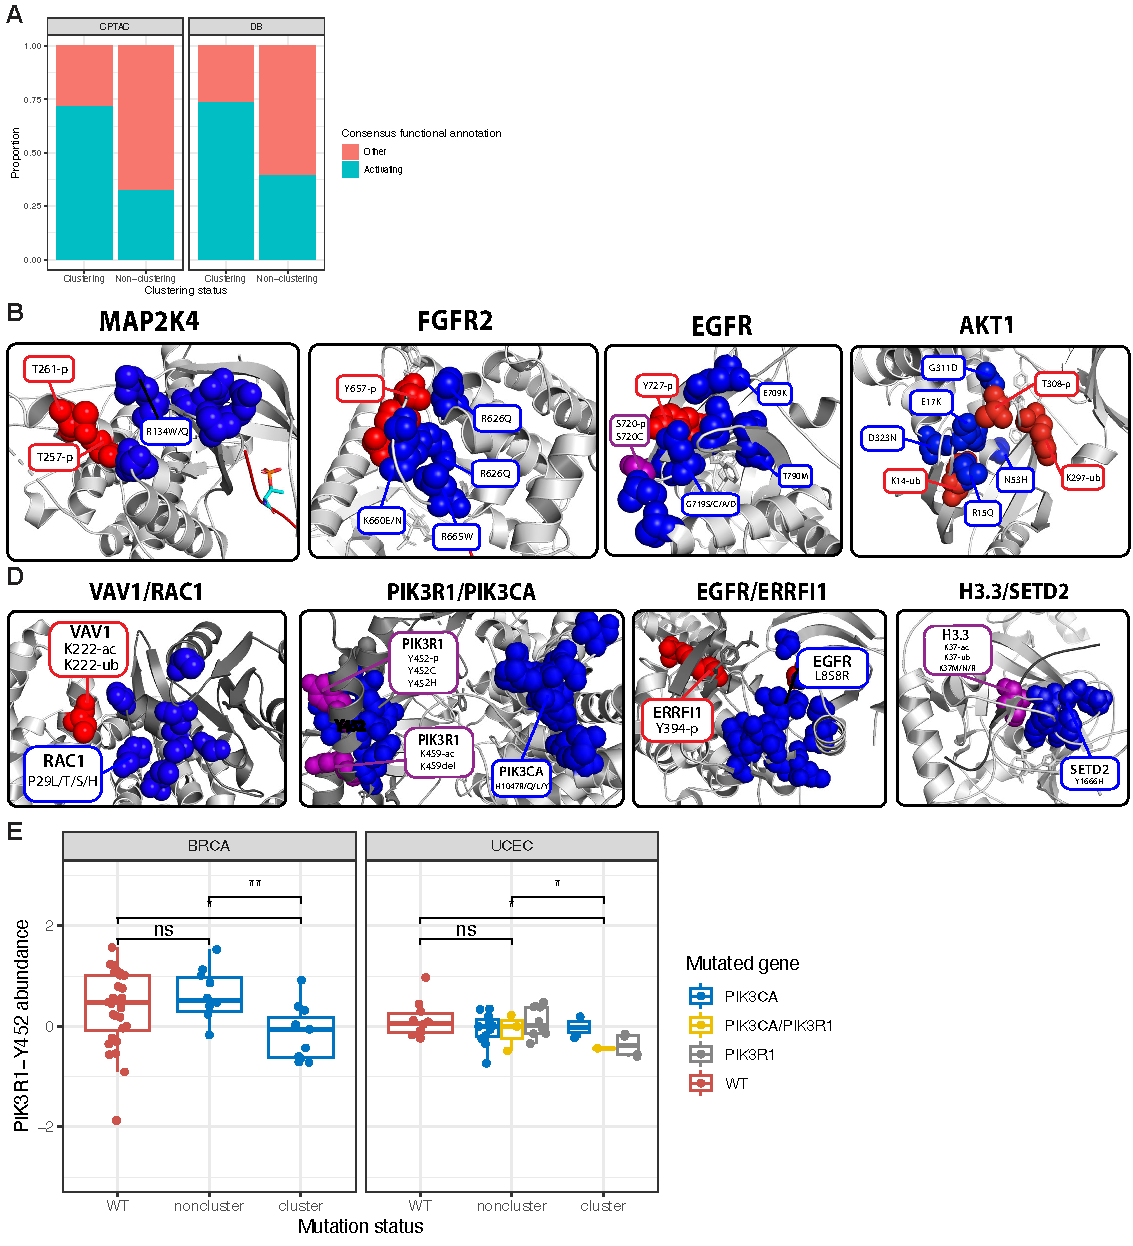
\includegraphics[width=\linewidth]{figures/chap03_ptmcosmos/figure6_ptmcosmos_hotptm.pdf}
    \caption[Spatial co-clustering of mutations and PTMs.]{%
        Spatial co-clustering of mutations and PTMs.
        \legendcontdnote
    }
    \label{fig:ptmcosmos-hotptm}
\end{figure}
\begin{figure}[t]
    \centering
    \legend{%
        \legendcontdref{fig:ptmcosmos-hotptm}
        \subref{fig:ptmcosmos-hotptm-enrich}
        Enrichment of activating mutations among mutations co-clustering with PTMs.
        \subref{fig:ptmcosmos-hotptm-structure}
        Selected mutation-PTM clusters mapped onto crystal structures obtained from the Protein Data Bank. Red spheres represent the residues modified by PTM sites, while blue spheres represent the residues affected by mutations.
        \subref{fig:ptmcosmos-hotptm-structure-complex}
        Visualization of mutation-PTM clusters spanning protein complexes. Purple spheres represent residues affected by both PTM sites and mutations.
        \subref{fig:ptmcosmos-hotptm-pi3k}
        Relative abundance of the PIK3R1-Y452 phosphosite in BRCA and UCEC stratified by mutation co-clustering status.
    }
\end{figure}

Of these hybrid clusters of interest, 41 were phosphosite-mutation clusters, 16 were ubiquitylsite-mutation clusters and 12 were acetylsite-mutation clusters. Interestingly, 36 clusters consisted of multiple PTM types in the same cluster, 15 of which featured acetylsites, ubiquitylsites and phosphosites in the same cluster. EGFR, ALB and CTNNB1 were the three genes with the greatest number of clusters, followed by TP53, PIK3R1 and B2M. The majority of clusters (89 out of 105) were confined to single proteins, with 16 clusters showing mutation-PTM clustering across protein complexes. Additionally, we used experimental data from Ba/F3 and MCF10A cell lines \cite{ngpks_millsgb:SystematicFunctional2018} to evaluate the functionality of co-clustering mutations (\fref{fig:ptmcosmos-hotptm-enrich}). Intriguingly, 71.7\% (66/92) of co-clustering mutations were activating compared to 32.4\% (154/476) of non co-clustering mutations (One-tailed Fisher's exact test, p = 2.3e-12). These findings are consistent with previous studies from our group investigating spatially interacting mutations and phosphosites, and suggest that mutations which co-cluster with ubiquityl- and acetylsites are enriched for activating mutations as well \cite{huangk_dingl:SpatiallyInteracting2021}. On the level of individual genes, co-clustering mutations were enriched for activating mutations for PIK3CA (p = 1.85e-4) and EGFR (p = 2.0e-3).

Next, we investigated the PTM sites co-clustering with known activating mutations in greater detail (\fref{fig:ptmcosmos-hotptm-structure}). Acetylation of IDH1 at K270 and IDH2 at K309 clustered with the canonical gain-of-function mutations at R132 and R172, respectively \cite{dangl_susm:CancerassociatedIDH12009,lemonnierf_maktw:IDH2R172K2016}. Phosphorylation of KRAS at Y32 and T35 co-clustered with mutations at the hotspot residues G12, A59 and Q61 \cite{hobbsga_rossmankl:RASIsoforms2016}. MAP2K4 phosphorylation at its activation sites of S257 and T261 co-clustered with high-frequency mutations at R134, consistent with previous studies finding that this residue interacts with both activation sites \cite{shevchenkoe_pantsart:AutoinhibitedState2020}. MAP2K1 ubiquitination at residues K168 and K175 clustered with the G128D mutation, known to result in MAPK pathway activation \cite{gaoj_sanderc:3DClusters2017}. Phosphorylation of CTNNB1 at S389 clustered with mutations known to disrupt APC binding and increase beta-catenin signaling \cite{liup_smitsr:OncogenicMutations2020}. The D194Y mutation in STK11, a known loss-of-function mutation which promotes tumor growth, clustered with phosphorylation at Y60 \cite{granado-martinezp_recioja:STK11LKB12020}. Although the function of several of these PTM sites is unclear, their co-clustering with activating mutations nominates them as promising targets for future investigation.

Additionally, our analysis revealed several novel clusters in the key driver genes TP53 and EGFR. Multiple PTM sites of TP53 co-clustered with distinct sets of activating mutations. Ubiquitination at K139 clustered with multiple mutations, including the directly overlapping K139N mutation, and the V143A mutation known to affect promoter binding \cite{friedlanderp_orenm:MutantP531996}. The TP53 phosphosite T150, known to be phosphorylated by the COP9 signalosome, clustered with several TP53 mutations, including the hotspot mutation V157F \cite{bech-otschird_dubielw:COP9Signalosomespecific2001,woohg_thorgeirssonss:AssociationTP532011}. The ubiquityl- and acetylsite K132 co-clustered with multiple mutations, including directly overlapping mutations, and mutations at the hotspot residues R248, R249 and R273.  Similarly, acetylation and ubiquitination at K120 clustered with the directly overlapping K120E and K120Q mutations, as well as canonical hotspot mutations such as R175H and G245S \cite{melloss_attardild:NotAll2013}. Interestingly, acetylation of K120 is known to increase p53-mediated transcription of pro-apoptotic genes, and thus cell death, suggesting that co-clustering mutations may disrupt this PTM site \cite{reedsm_quellede:P53Acetylation2014}. EGFR also exhibited several mutation-PTM clusters involving functional mutations. Interestingly, phosphorylation of EGFR at Y727, known to result in SHC binding and potentially downstream signaling, clustered with G719 and E709K mutations known to affect sensitivity to tyrosine kinase inhibitors, and the T790M mutation known to result in drug resistance \cite{zhangt_songy:TreatmentUncommon2019,yunch_eckmj:T790MMutation2008,harrisonpt_huangph:RareEpidermal2020}. The acetylation sites K261 and K293 co-clustered with distinct sets of mutations, including extracellular domain mutations known to increase receptor sensitivity to ligand stimulation \cite{hoogstratey_frenchpj:EGFRMutations2020}. Intriguingly, phosphorylation at Y1016, known to activate downstream signalling, clustered with multiple exon 20 mutations, including the previously reported S768I missense mutation, known to be responsive to EGFR inhibitors \cite{kanchark_duysterj:FunctionalAnalysis2009,lundbya_olsenjv:OncogenicMutations2019}. The spatial co-clustering of these mutations and the Y1016 autophosphosite require further investigation to determine if these mutations can promote EGFR activity through interacting with the phosphotyrosine residue.

Intriguingly, several hybrid clusters highlighted potential mechanisms of kinase activation through mutation-PTM crosstalk. Phosphorylation of FGFR2 at Y657, known to be crucial for its activation, clustered with multiple mutations at K660 \cite{chenh_mohammadim:MolecularBrake2007}. Previous studies have implicated K660 mutations in shifting FGFR2 from an auto-inhibited to activated state, suggesting that mutations at this residue may promote FGFR2 activation through interacting with the Y657 phosphosite \cite{greulichh_pollockpm:TargetingMutant2011}. Additionally, the AKT1 mutation E17K was clustered with the K14 and K297 ubiquitylsites, as well as the activating phosphosite T308, consistent with E17K resulting in increased ubiquitination of AKT1 and driving kinase activation through T308 phosphorylation \cite{yangwl_linhk:RegulationAkt2010}. In particular, ubiquitination of AKT1 at K14 is known to promote phosphorylation at T308, suggesting that the spatial co-clustering of these PTM sites and mutations promotes AKT1 activation \cite{yangwl_linhk:E3Ligase2009}.

In addition, several clusters featured directly overlapping PTM sites and mutations. These included the canonical N-terminal hotspot mutations in CTNNB1 co-clustering with phosphorylation of Y30, S33 and T40 through T42. Residue K22 of CDK4, known to be important for cyclin D binding, exhibited both ubiquitination and mutations, including mutations known to affect kinase activity \cite{lij_tsaimd:DissectionCDK4Binding2005}. Acetylation of the splicing factor SF3B1 at K700 directly overlapped with the K700E mutation, known to dysregulate SF3B1-mediated splicing \cite{obengea_ebertbl:PhysiologicExpression2016}. The S249C mutation of FGFR3, known to result in constitutive receptor activation, overlapped with phosphorylation at the same site \cite{limanc_huangph:TargetingSrc2020}. Ubiquitination of KRAS at K117 clustered with K117N and A146T mutations, known to promote KRAS activity and ERK phosphorylation, although to a lesser degree than G12D mutations \cite{stolzeb_schollc:ComparativeAnalysis2015,janakiramanm_solitdb:GenomicBiological2010}. Phosphorylation of RAF1 at S259, important for RAF1 inhibition through 14-3-3 protein binding, clustered with S259F and S257L mutations known to increase kinase activity \cite{panditb_gelbbd:GainoffunctionRAF12007}. Thus, the direct overlap of mutations and PTM sites may indicate potential mutation-PTM crosstalk with biological implications.

Moreover, we observed several mutation-PTM clusters spanning protein complexes.
Notably, phosphorylation of the tumor suppressor Mig6 at Y394 co-clustered with multiple \gene{EGFR} mutations and PTM sites. Previous studies have elucidated the role of this phosphosite in promoting the degradation of wild-type, but not \gene{EGFR} mutant, consistent with the Y394 phosphosite clustering with activating EGFR mutations such as L858R and L861Q \cite{gazdaraf_gazdaraf:ActivatingResistance2009,kanchark_duysterj:EpidermalGrowth2011,maitytk_guhau:LossMIG62015}. Interestingly, this cluster also included the EGFR ubiquitination sites at K846 and K875 in the activation loop, with the former site implicated in activating \gene{EGFR} mutant and the latter site possibly playing a role in receptor trafficking \cite{rayp_rayd:UbiquitinLigase2020}. Thus, these results suggest that the spatial proximity of EGFR mutations and Mig6 phosphorylation sites may promote EGFR stability. Additionally, acetylation of the guanine nucleotide exchange factor VAV1 at K222, known to disrupt its adaptor role in signaling, clustered with activating mutations in the GTPase RAC1 at residue P29 \cite{dep_deyn:RAC1Takes2019,rodriguez-fdezs_busteloxr:LysineAcetylation2020}. Interestingly, ubiquitination at residue K37 of the histone H3F3A (H3.3), known to prime H3 acetylation and affect gene expression, overlapped with K37R and K37N mutations. This H3.3 residue also clustered with mutations in the histone methyltransferase SETD2, including mutation of residue Y1666 to histidine \cite{zhangx_linhk:H3Ubiquitination2017}. Notably, this residue of SETD2 is known to be important for the SETD2-H3.3 interaction, suggesting that the interaction of residues K37 of H3.3 and Y1666 of SETD2 may have biological significance \cite{yangs_lih:MolecularBasis2016}. Phosphorylation and acetylation of PIK3R1 at Y452 and K459, respectively, overlapped with mutations at these residues (Y452H and K459del), as well as with known oncogenic mutations in PIK3CA, including at the hotspot residue H1047 \cite{vasann_baselgaj:DoublePIK3CA2019}. Thus, our analysis highlights multiple mutation-PTM clusters across driver gene complexes which may be promising targets for functional studies.

Due to the spatial proximity of the PIK3R1-Y452 phosphosite to PIK3CA, we chose to further investigate the potential biological role of this site (\fref{fig:ptmcosmos-hotptm-pi3k}). First, we analyzed the association of co-clustering mutations with PIK3R1-Y452 abundance. Samples with co-clustering mutations displayed lower phosphorylation of PIK3R1 at Y452 in UCEC tumors, consistent with these mutations including overlapping mutations (Y452H, K459del) that may disrupt phosphorylation at this residue. Interestingly, BRCA tumors showed a similar but more significant trend (p = 0.0063, Wilcoxon rank-sum test), with co-clustering mutations in this cohort consisting solely of PIK3CA mutations. The vast majority (17/19) of these mutations were at the hotspot residue H1047, suggesting that oncogenic mutations in PIK3CA may affect phosphorylation of PIK3R1 at Y452. Strikingly, in both cohorts, samples with clustering mutations showed lower PIK3R1-Y452 phosphorylation than both samples with non-clustering mutations in \gene{PIK3R1} or \gene{PIK3CA}, and samples lacking mutations in either gene (hereafter called wildtype samples), further suggesting that these co-clustering mutations may affect Y452 phosphorylation. Interestingly, in UCEC, both clustering and non-clustering mutations showed lower PIK3CA protein abundance. Compared to UCEC wildtype samples, samples with co-clustering \gene{PIK3R1} mutations showed a more significant decrease in PIK3CA protein abundance than samples with co-clustering PIK3CA mutations. Furthermore, we analyzed the correlations between PIK3R1-Y452 abundance and PIK3CA protein abundance across cancer types. Intriguingly, across GBM tumors PIK3R1-Y452 abundance was significantly correlated with PIK3CA protein abundance (R = 0.47, p = 0.011), but not with PIK3R1 protein abundance (R = 0.17, p = 0.4), suggesting that phosphorylation at this site may affect the PIK3R1-PIK3CA interaction. We observed a similar, although less significant, trend across UCEC tumors, with PIK3R1-Y452 abundance showing a weak association with PIK3R1 protein abundance (R = -0.14, p = 0.41) and stronger correlation with PIK3CA protein abundance (R = 0.31, p = 0.057). Thus, PIK3R1-Y452 may be a promising phosphosite for further investigation and experimental evaluation.


\subsection{Database only spatial mutation-PTM clusters by HotPTM}
To understand the spatial clustering of PTMs not detected in CPTAC, we ran HotSpot3D on 1,072,389 TCGA MC3 and CPTAC mutations and 14,054 driver gene PTM sites in PTMcosmos to obtain 28,741 total mutation-PTM, PTM-PTM and mutation-mutation clusters. Selecting the mutation-PTM (hybrid) clusters in the top 5\% of cluster closeness scores resulted in 57 clusters of interest. Interestingly, 32 clusters contained multiple different PTM types in the  same cluster, consisting largely of phospho/ubiquityl, acetyl/phospho/ubiquityl and acetyl/methyl/phospho/ubiquityl clusters. TP53, CTNNB1 and PIK3R1 were the three most represented genes among the clusters of interest, and 51 out of the 57 clusters were confined to single proteins. Similar to the CPTAC clusters, 78.5\% (95 out of 121) of the co-clustering mutations were activating compared to 35.9\% (166 out of 463) of non co-clustering mutations, suggesting that mutation-PTM clusters are universally enriched for activating mutations.

The hybrid clusters of interest obtained from PTMcosmos sites included several not found when using only CPTAC sites. Notably, several clusters exhibited co-clustering between ubiquitylsites and phosphosites of known function. The K291 and K292 ubiquitylsites of p53, known to promote its proteasomal degradation, co-clustered with the S215 phosphosite, known to inactivate and destabilize wildtype p53 \cite{fraserja_hupptr:NovelP532010}. The K291 ubiquitylsite of p53 also co-clustered with the K164 acetylsite, known to in part inhibit repression of p53 by Mdm2 \cite{yt_wg:AcetylationIndispensable2008}. Similarly, the Mdm2- and Pirh2-targeted K101 ubiquitylsite of p53 clustered with the T211 phosphosite, known to in part promote proteasomal degradation of p53 \cite{gullycp_leemh:AuroraKinase2012,shloushj_arrowsmithch:StructuralFunctional2011}. Interestingly, the S305 phosphosite of caspase-8, known to inhibit apoptosis \cite{matthessy_strebhardtk:SequentialCdk12014}, co-clustered with several ubiquitylsites (K224, K229, K461) known to inhibit caspase-8 activity through promoting its proteasomal degradation \cite{gonzalvezf_ashkenazia:TRAF2Sets2012}. Among the multi-protein clusters, the K64 ubiquitylsite of Nrf2 co-clustered with the S602 phosphosite of Keap1 at the binding interface of these proteins \cite{cloerew_majormb:NRF2Activation2019}. Notably, these PTM sites co-clustered with oncogenic mutations in the Keap1 binding domain of Nrf2, suggesting that these PTM sites may play a role in the Keap1-Nrf2 interaction.



\section{Discussion}



\section{Methods}

\subsection{Data sources}
\subsubsection{CPTAC proteomic data processing}

\tref{tab:ptmcosmos-peptide-db} \url{https://github.com/ccwang002/cptac_proteome_preprocess}


\begin{table}[tbp]
    \centering
    \caption{CPTAC peptide search databases used by different disease working group.}
    \label{tab:ptmcosmos-peptide-db}
    \begin{threeparttable}[b]
    \begin{tabular}{@{}llll@{}}
    \toprule
    Phase & Cohort & Database & Notes \\
    \midrule
    \multirow{2}{*}{\begin{tabular}[c]{@{}l@{}}CPTAC2/TCGA\\ retrospective\end{tabular}}
        & BRCA  & RefSeq 20130727   & Broad Institute \\
        & OV    & RefSeq 20111201   & PNNL \\
    \midrule
    \multirow{3}{*}{\begin{tabular}[c]{@{}l@{}}CPTAC2\\ prospective\end{tabular}}
        & OV    & CDAP (Refseq 2016)    & PNNL \\
        & CRC   & RefSeq 20171003\tnote{*}  & Use RefSeq 2018 instead \\
        & BRCA  & CDAP (Refseq 2016)    & Broad Institute \\
    \midrule
    \multirow{8}{*}{\begin{tabular}[c]{@{}l@{}}CPTAC3\\ discovery\end{tabular}}
        & CCRCC & CDAP (Refseq 2018) & UMich \\
        & GBM   & CDAP (Refseq 2018) & PNNL \\
        & HNSCC & CDAP (Refseq 2018) & UMich \\
        & LUAD  & CDAP (Refseq 2018)\tnote{\textdagger} & Broad Institute \\
        & LSCC  & CDAP (Refseq 2018)\tnote{\textdagger} & Broad Institute \\
        & PBTA  & CDAP (Refseq 2018) & MS3 spectra \\
        & PDAC  & CDAP (Refseq 2018) & UMich \\
        & UCEC  & CDAP (Refseq 2018) & PNNL \\
    \bottomrule
    \end{tabular}
    \begin{tablenotes}
    \item [*] Database uses hg38 genome reference.
    \item [\textdagger] Database includes smORFs.
    \end{tablenotes}
    \end{threeparttable}
\end{table}


\subsubsection{PTM coordinate harmonization and protein sequence alignment}
Only considered the canonical reviewed UniProt entries
If the identical protein sequence can be found, mapped to them directly
Otherwise, perform global protein sequence alignment
To the UniProt entry of the same gene
Create coordinate segments of consecutive matches (don't allow any amino acid mismatch)
Only mapped the site when a full peptide (plus the 1 additional flanking aa) is in the coordinate segment

\subsection{Database and website development}

\chapter{CPTAC Glioblastoma Discovery Study}
\label{chap:cptac-gbm-discov}

% This chapter describes work published at https://doi.org/10.1016/j.ccell.2021.01.006
% i need fig1, fig2a/b, fig 4 a/d-f, fig 5a, fig 7a/c.

\begin{figure}[tbp]
    \centering
    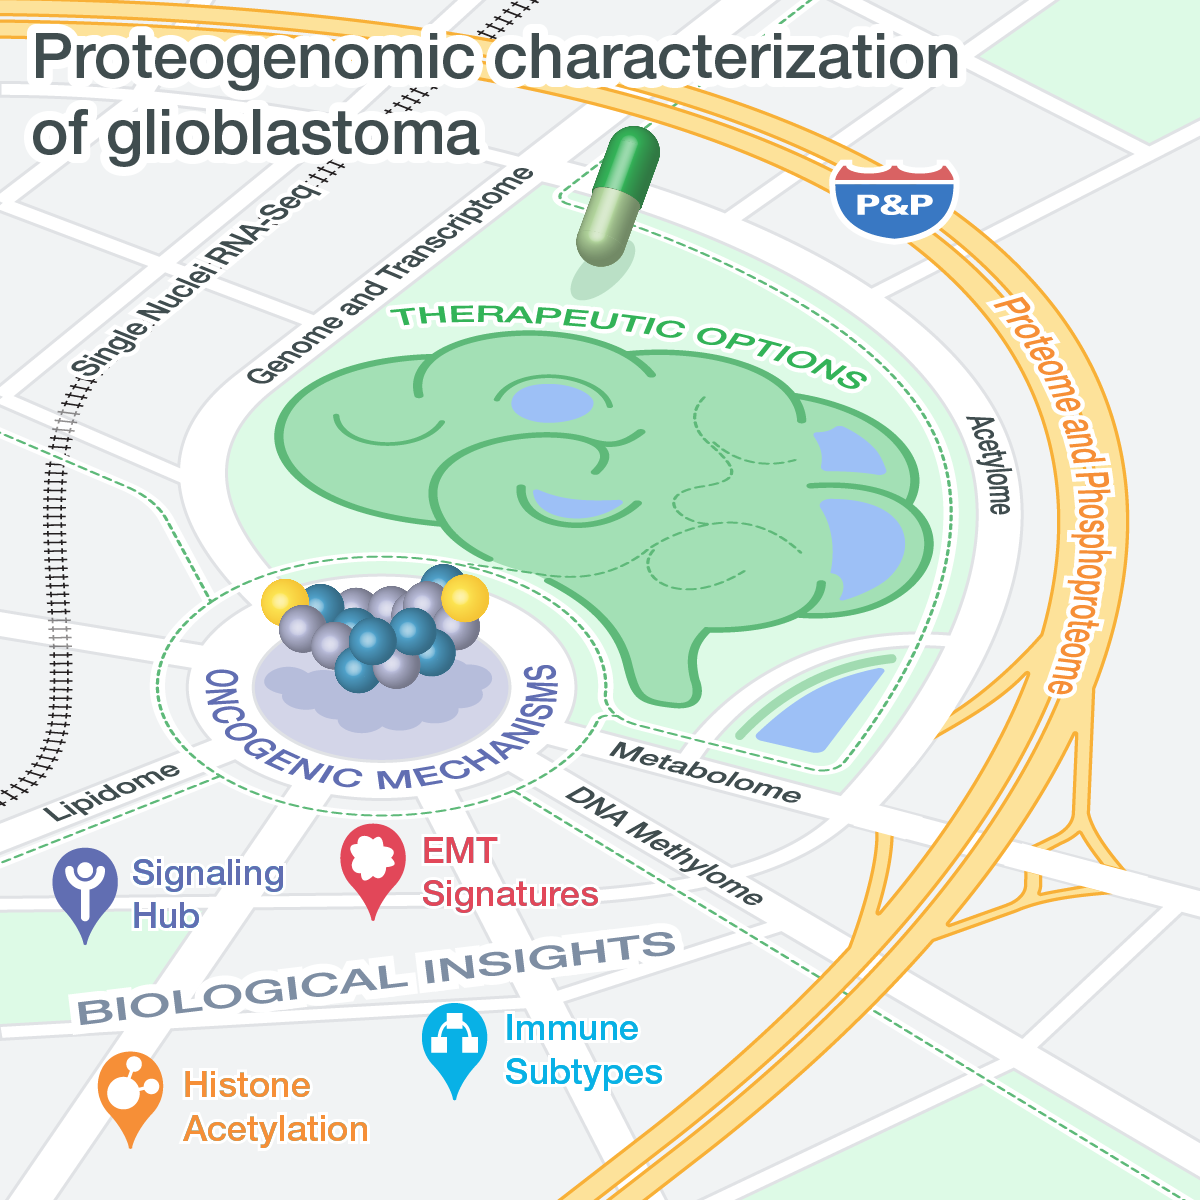
\includegraphics[height=0.5\textheight]{figures/chap04_cptac_gbm_discov/graphical_abstract.png}
    \caption{Graphical abstract of the CPTAC GBM discovery study.}
    \label{fig:gbm-graphical-abstract}
\end{figure}

\section{Summary}
Glioblastoma (GBM) is the most aggressive nervous system cancer. Understanding its molecular pathogenesis is crucial to improving diagnosis and treatment. Integrated analysis of genomic, proteomic, post-translational modification and metabolomic data on 99 treatment-naive GBMs provides insights to GBM biology. We identify key phosphorylation events (e.g., phosphorylated PTPN11 and PLCG1) as potential switches mediating oncogenic pathway activation, as well as potential targets for \gene{EGFR}-, \gene{TP53}-, and RB1-altered tumors. Immune subtypes with distinct immune cell types are discovered using bulk omics methodologies, validated by snRNA-seq, and correlated with specific expression and histone acetylation patterns. Histone H2B acetylation in classical-like and immune-low GBM is driven largely by BRDs, CREBBP, and EP300. Integrated metabolomic and proteomic data identify specific lipid distributions across subtypes and distinct global metabolic changes in \gene{IDH}-mutated tumors. This work highlights biological relationships that could contribute to stratification of GBM patients for more effective treatment.

\section{Introduction}
Glioblastoma (GBM) is the most common primary malignant brain tumor, with roughly 12,000 new cases annually in the United States and median survival under 2 years \cite{delgado-lopezpd_corrales-garciaem:SurvivalGlioblastoma2016,ostromqt_barnholtz-sloanjs:CBTRUSStatistical2019}. The Cancer Genome Atlas (TCGA) \cite{brennancw_chinl:GBM2013,tcga_network:GBM2008} and other studies \cite{yanh_bignerdd:IDH1IDH22009} have reshaped the World Health Organization classification of nervous system tumors \cite{louisdn_ellisondw:2016World2016} to include molecular features \cite{bratdj_wellerm:CIMPACTNOWUpdate2018, louisdn_vondeimlinga:AnnouncingCIMPACTNOW2017}.
GBM is categorized as either \gene{IDH}-wild type (\gene{IDH}-WT; \textasciitilde90\%) or \gene{IDH}-mutant (\textasciitilde10\%). \gene{IDH}-WT GBMs fall into three distinct subclasses (proneural, classical, and mesenchymal) based on genomic alterations and gene expression signatures \cite{verhaakrgw_hayesdn:IntegratedGenomic2010,wangq_verhaakrgw:TumorEvolution2017}. Methylome-based classification is being used to differentially diagnose brain tumors \cite{karimis_zadehg:CentralNervous2019,nassirif_aldapekd:DNAMethylation2019} and may become clinically useful for GBM.
Surgical resection, chemotherapy, and radiotherapy remain the standard of care \cite{stuppr_mirimanoffro:RadiotherapyConcomitant2005,perryjr_trialinvestigators:ShortCourseRadiation2017}, with the recent addition of tumor treating fields \cite{stuppr_ramz:EffectTumorTreating2017}.
Promising immunotherapies have been proposed, including immune checkpoint inhibitors, vaccines, chimeric antigen receptor T cell (CAR-T) therapy, and viral therapy, though none have cleared Phase III trials \cite{limm_wellerm:CurrentState2018,mcgranahant_nagpals:CurrentState2019}.
Despite different subtypes, no specific treatment works more effectively in a pre-specified subset of patients based on transcriptomics, though those with MGMT promoter methylation respond better to temozolomide \cite{stuppr_mirimanoffro:RadiotherapyConcomitant2005}.

Here, we integrated proteogenomic and metabolomic data from 10 platforms including whole genome sequencing (WGS), whole exome sequencing (WES), RNA sequencing (RNA-seq), microRNA-seq (miRNA-seq), single nuclei RNA-seq (snRNA-seq), DNA methylation arrays, proteome, phosphoproteome, acetylome, lipidome, and metabolome to investigate 99 treatment-naive GBMs prospectively collected by the Clinical Proteomic Tumor Analysis Consortium (CPTAC). We report new immune-based subtypes, activation of DNA repair pathways via upregulated phosphosite levels of DNA repair genes in \gene{TP53}-mutated tumors, an apparent phospho-signaling bottleneck in receptor tyrosine kinase (RTK)-altered tumors, and enrichment of histone H2B acetylation and low macrophage content in classical-like GBM tumors. We used single-cell data to investigate contributions of various cell types to bulk tumor signatures and analyzed the mesenchymal subtype to discern epithelial-mesenchymal transition (EMT) signatures in tumor and infiltrating immune cells. The data presented here furnish a resource for future GBM studies.

\chapter{Ongoing GBM single cell analysis and CPTAC GBM confirmatory cohort}
\label{chap:gbm-single-cell}

\chapter{Conclusion and Future Directions}
\label{chap:conclusion}
% Discussion: remaining challenges, the benefits in another fields than oncology


\begin{SingleSpace}
% \nocite{*}
\printbibliography
\end{SingleSpace}

\appendix
\chapter{Open Source Tool and Pipeline Development}
\label{app:oss-pipeline-dev}


\end{document}
